\documentclass[12pt,modern,twocolumn,tighten]{aastex63}
%\documentclass[12pt,twocolumn,tighten,linenumbers]{aastex63}
%\documentclass[12pt,twocolumn,tighten,trackchanges]{aastex63}
\usepackage{amsmath,amstext,amssymb}
\usepackage[T1]{fontenc}
\usepackage{apjfonts}
\usepackage[figure,figure*]{hypcap}
\usepackage{graphics,graphicx}
\usepackage{hyperref}
\usepackage{natbib}
\usepackage[caption=false]{subfig} % for subfloat
\usepackage{enumitem} % for specific spacing of enumerate
\usepackage{epigraph}

\renewcommand*{\sectionautorefname}{Section} %for \autoref
\renewcommand*{\subsectionautorefname}{Section} %for \autoref

\newcommand{\cn}{$\delta$\ Lyr\ cluster} % cluster name
\newcommand{\sn}{Kepler\,1627} % star system name (binary)
\newcommand{\pn}{Kepler\,1627Ab} % planet name

\newcommand{\clusterage}{$38^{+6}_{-5}$\,Myr} % 

% gaia target sample numbers
\newcommand{\nkinematic}{1{,}201} % deltalyr_kc19_cleansubset_withreddening.csv
% all from oneoff_calculate_rotation_numbers.py
\newcommand{\noriginal}{3{,}071} % Vizier; KC19 Theia 73 member count
\newcommand{\nwithtess}{924} % How many stars have TESS data with G<17 and (Bp-Rp)0 > 0.5?
\newcommand{\nforgyro}{1842} % How many stars have G<17 and (Bp-Rp)0 > 0.5?
\newcommand{\nkinwithtess}{391} % How many kinematically selected stars have TESS data?
\newcommand{\nkinwithtessandcrowding}{192} % How many kinematically selected stars have TESS data and meeting the crowding cutoff (nequal<=0, nclose<=1)?
\newcommand{\nkindefaultcleaning}{145} % How many of these meet the "defaultcleaning" criteria (LSP>0.1, Prot<15, and crowding cut)?
\newcommand{\nrotgood}{135} % nkindefaultcleaning, minus outliers.
\newcommand{\nfracprot}{70} % fraction nrotgood/nkinwithtessandcrowding


%
% Symbols
%
\newcommand{\kms}{\,km\,s$^{-1}$}
\newcommand{\ms}{\,m\,s$^{-1}$}
\newcommand{\bpmrpo}{(G_{\rm BP}-G_{\rm RP})_0}
\newcommand{\bpmrp}{G_{\rm BP}-G_{\rm RP}}

%% Reintroduced the \received and \accepted commands from AASTeX v5.2.
%% Add "Submitted to " argument.
\received{---}
\revised{---}
\accepted{---}
\submitjournal{AAS Journals}
\shorttitle{Kepler\,1627}

\begin{document}

\title{
  %Kepler 1627Ab: A 38 Million Year Old
  %Kepler 1627 Ab:
  %A Mini-Neptune in the Kepler Field Only 38 Million Years Old
  A 38 Million Year Old Mini-Neptune in the Kepler Field
}

%\suppressAffiliations
%\NewPageAfterKeywords
\correspondingauthor{L.\,G.\,Bouma}
\email{bouma.luke@gmail.com}

\author[0000-0002-0514-5538]{L. G. Bouma}
\affiliation{Department of Astrophysical Sciences, Princeton University, 4 Ivy Lane, Princeton, NJ 08540, USA}

% Key authors:
% ... stellar rotation & the initial crossmatch
\author[0000-0002-2792-134X]{J. L. Curtis}
\affiliation{Department of Astronomy, Columbia University, 550 West 120th Street, New York, NY 10027, USA}
\affiliation{Department of Astrophysics, American Museum of Natural History, New York, NY 10024, USA}

% ... Kepler correlations
\author[0000-0003-1298-9699]{K. Masuda}
\affiliation{Department of Earth and Space Science, Osaka University, Osaka 560-0043, Japan}

% ... HIRES PI
\author{L. A. Hillenbrand}
\affiliation{Cahill Center for Astrophysics, California Institute of Technology, Pasadena, CA 91125, USA}

% ... RM fitting
\author[0000-0001-7409-5688]{G. Stefansson}
\affiliation{Department of Astrophysical Sciences, Princeton University, 4 Ivy Lane, Princeton, NJ 08540, USA}

%
% PFS Collaborators
%
\author[0000-0001-8638-0320]{A. W. Howard}
\affiliation{Cahill Center for Astrophysics, California Institute of Technology, Pasadena, CA 91125, USA}
%
\author[0000-0002-0531-1073]{H. Isaacson}
\affiliation{Astronomy Department, University of California, Berkeley,
CA 94720, USA}

%
% MUSCAT3 Collaborators
%
\author[0000-0001-8511-2981]{N. Narita}
\affiliation{Komaba Institute for Science, The University of Tokyo, Tokyo 153-8902, Japan}
\affiliation{Japan Science and Technology Agency, PRESTO, Tokyo 153-8902, Japan}
\affiliation{Astrobiology Center, Tokyo 181-8588, Japan}
\affiliation{Instituto de Astrof\'{i}sica de Canarias (IAC), 38205 La Laguna, Tenerife, Spain}

\author[0000-0002-4909-5763]{A. Fukui} % afukui@g.ecc.u-tokyo.ac.jp
\affiliation{Komaba Institute for Science, The University of Tokyo, Tokyo 153-8902, Japan}
\affiliation{Instituto de Astrof\'{i}sica de Canarias (IAC), 38205 La Laguna, Tenerife, Spain}

\author[0000-0002-5658-5971]{Masahiro Ikoma} % ikoma.masahiro@gmail.com
\affiliation{Division of Science, National Astronomical Observatory of Japan, Tokyo 181-8588, Japan}

\author[0000-0002-6510-0681]{M. Tamura} % motohide.tamura@nao.ac.jp
\affiliation{Department of Astronomy, University of Tokyo, Tokyo 113-0033, Japan}
\affiliation{Astrobiology Center, Tokyo 181-8588, Japan}
\affiliation{National Astronomical Observatory of Japan, Tokyo 181-8588, Japan}

% AO IMAGING
\author[0000-0001-9800-6248]{E. Furlan} % furlan@ipac.caltech.edu
\affiliation{NASA Exoplanet Science Institute, Caltech/IPAC, Pasadena, CA 91125, USA}

\author[0000-0003-2519-6161]{C.~L.~Gnilka} % clgnilka@gmail.com
\affiliation{NASA Ames Research Center, Moffett Field, CA 94035, USA}

\author[0000-0002-9903-9911]{K.~V.~Lester} % klester192@gmail.com
\affiliation{NASA Ames Research Center, Moffett Field, CA 94035, USA}

\author[0000-0002-2532-2853]{S. B. Howell}
\affiliation{NASA Ames Research Center, Moffett Field, CA 94035, USA}




% 208 words (250 max)
\begin{abstract}
  Kepler\,1627A is a G8V star previously known to host a
  $3.4\,R_\oplus$ mini-Neptune on a 7.2\,day orbit.  The star was
  observed by the Kepler space telescope because it is nearby
  ($d=329\,{\rm pc}$) and it resembles the Sun.  Here we show
  using Gaia kinematics, TESS stellar rotation periods, and
  spectroscopic lithium abundances that Kepler\,1627 is a member of
  the \clusterage\ old $\delta$~Lyr cluster.  To our knowledge, this makes
  Kepler\,1627Ab the youngest planet with a precise age yet found
  by the main Kepler mission.
  The Kepler photometry shows two 
  peculiarities: the average transit profile appears to be
  asymmetric, and the individual transit times are correlated with the
  local light curve slope.
  We discuss possible explanations for each anomaly.
  More widely applicable though is the fact that the $\delta$~Lyr
  cluster is one of $\sim$10$^3$ clusters whose properties have been
  clarified by Gaia.  Many other exoplanet hosts are candidate
  members of these clusters based on kinematics; their ages can
  be confirmed by using the TESS full frame images to
  measure stellar rotation periods.
\end{abstract}

\keywords{
  exoplanet evolution (491),
  open star clusters (1160),
	stellar ages (1581)
}

%%%%%%%%%%%%%%%%%%%%%%%%%%%%%%%%%%%%%%%%%%%%%%%%%%%%%%%%%%%%%%%%%%%%%%%%%%%%%%%


\section{Introduction}

While thousands of exoplanets have been discovered orbiting nearby
stars, the vast majority of them are several billion years old.  This
makes it difficult to test origin theories for the different families
of planets, since many evolutionary processes are expected to operate
on timescales of less than 100 million years.

%TODO: might want to revise this text to better frame the boil-off phase...
%TODO: better citations on radius evolution?
For instance, the ``mini-Neptunes'', thought to be made of molten
rocky cores \citep{kite_atmosphere_2020} and extended atmospheric
envelopes of hydrogen and helium, are expected to shrink in size by
factors of several over their first $10^8$ years.  Specifically, in
the models of \citet{owen_atmospheres_2016} and
\citet{owen_constraining_2020}, the $\approx5\,M_\oplus$ planets start
with sizes of 4--12\,$R_\oplus$ shortly after the time of disk
dispersal ($\lesssim$$10^7$\,years), and shrink to sizes of
2--4\,$R_\oplus$ by 10$^8$ years.  While the majority of this change
is expected to occur within the first few million years after disk
dispersal \citep{owen_atmospheres_2016}, the combination of stellar
irradiation and internal heat may also power a more gradual outflow
which can eventually deplete or entirely strip the envelope from the
rocky core \citep{Owen_Wu_2013,ginzburg_corepowered_2018}.
Discovering young planets, measuring their masses, and detecting their
atmospheric outflows are key steps toward testing this paradigm, which
is often invoked to explain the observed radius distribution of mature
exoplanets \citep{Fulton_et_al_2017}.

The K2 and TESS missions have now enabled the detection of about ten
close-in planets younger than 100 million years, all smaller than
Jupiter
\citep{Mann_K2_33b_2016,David_et_al_2017,david_four_2019,newton_tess_2019,bouma_cluster_2020,plavchan_planet_2020,rizzuto_tess_2020,martioli_aumicbc_2021}.
The Kepler mission however has not yielded any planets with precise
ages below one gigayear \citep{Meibom_et_al_2013}.  The reason is that
during the main Kepler mission (2009--2013), only four open clusters
were known in the Kepler field,
%: NGC\,6866, NGC\,6811, NGC\,6819, and NGC\,6791,
with ages spanning 0.7\,Gyr to 9\,Gyr
\citep{meibom_kepler_2011}.  Though isochronal, gyrochronal, and lithium-based
analyses suggest that younger Kepler planets do exist
\citep{berger_identifying_2018,david_sizes_2021}, accurate and precise
age measurements typically require an ensemble of stars.  Fortunately,
recent analyses of the Gaia
data have greatly expanded our knowledge of cluster memberships
\citep[{\it
e.g.},][]{cantatgaudin_gaia_2018,zari_3d_2018,kounkel_untangling_2019,Meingast2021,Kerr2021}.
As part of our Cluster Difference Imaging Photometric Survey (CDIPS,
\citealt{bouma_cdipsI_2019}), we concatenated the available analyses
from the literature, which yielded a list of candidate young and
age-dated stars (see Appendix~\ref{app:targetlist}).

Matching our young star list against stars observed by Kepler revealed that
%two discoveries.  The first, to be discussed in an upcoming analysis
%by J.~Curtis et al{.}, is that Kepler observed the $\approx$350\,Myr
%open cluster Theia~520 (UBC~1).  At least six Kepler planets are known
%in the cluster from the Kepler-52 and Kepler-968 systems
%\citep{rowe_validation_2014,jontof-hutter_following_2021}.  The second
%discovery, and the focus of this work, is
Kepler observed a portion of the \cn\ (Stephenson-1;
Theia~73).
More specifically, a clustering analysis of the Gaia
data by \citet{kounkel_untangling_2019}
reported that Kepler~1627 (KIC 6184894; KOI 5245; TIC 120105470) is a
\cn\ member.  Given the
previous statistical validation of the close-in mini-Neptune Kepler
1627b
\citep{2012ApJS..199...24T,morton_false_2016,thompson_planetary_2018},
we begin by examining the properties of the cluster more
closely (Section~\ref{sec:cluster}).  We find that the $\delta$ Lyr
cluster is \clusterage\ old, and 
in 
Section~\ref{sec:stars} show
that \sn\ is both a binary and also a member of the cluster.
Focusing on the planet (Section~\ref{sec:planet}), we confirm that despite the
presence of the previously unreported M2.5V companion, hereafter
Kepler\,1627B, the planet orbits the G-dwarf primary, Kepler\,1627A.  Based on a correlation between the
planetary transit times and the local light curve slope, the orbit
may also be prograde.  We conclude by highlighting broader
implications for our ability to age-date a larger sample of planets
(Section~\ref{sec:conc}).




\section{The Cluster}
\label{sec:cluster}

\begin{figure*}[t]
	\begin{center}
		\leavevmode
		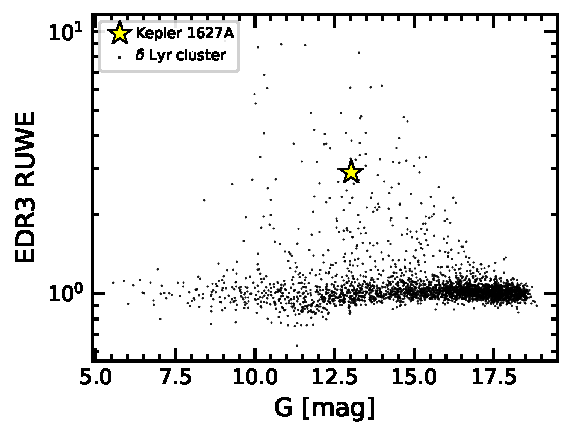
\includegraphics[width=1\textwidth]{f6.pdf}
	\end{center}
	\vspace{-0.7cm}
	\caption{
		{\bf Galactic positions and tangential velocities of stars in the
			$\delta$\,Lyr cluster.} Points are reported cluster members from
		\citet{kounkel_untangling_2019}.  
		The tangential velocities relative to
		\sn\ (lower-right) are computed assuming that every star has the same
		three-dimensional spatial velocity as \sn.
		Our analysis uses stars (black points)
		in the spatial and kinematic vicinity of Kepler\,1627 (yellow
		star).  The question of whether the other candidate cluster members
		(gray points) are part of the cluster is outside our scope.  The
		location of the Sun is ($\odot$) is shown.
		\label{fig:XYZvtang}
	}
\end{figure*}


To measure the age of the $\delta$ Lyr cluster, we first selected
a set of candidate cluster members
(Section~\ref{sec:kinematicselection}), and then analyzed these stars using a
combination of the isochronal and gyrochronal techniques
(Section~\ref{sec:clusterage}).


\subsection{Selecting Cluster Members}
\label{sec:kinematicselection}

\citet{kounkel_untangling_2019} applied an unsupervised clustering
algorithm to Gaia DR2 on-sky positions, proper motions, and
parallaxes for stars within the nearest kiloparsec.  For the \cn\
(Theia 73), they reported \noriginal\ candidate members.  We
matched these stars against the latest Gaia EDR3 observations using
the \texttt{dr2\_neighbourhood} table from the ESA archive\footnote{See
\url{https://gea.esac.esa.int/archive/documentation/GEDR3/Gaia_archive/chap_datamodel/sec_dm_auxiliary_tables/ssec_dm_dr2_neighbourhood.html}.},
and took the closest proper motion and epoch-corrected angular
distance as the presumed match
\citep{gaia_collaboration_2021_edr3}.  In Figure~\ref{fig:XYZvtang},
have shown galactic positions only for the stars with
parallax signal-to-noise exceeding 20.  The reported cluster members
(gray and black points) extend over a much larger volume than the
cluster previously identified by \citet{stephenson_possible_1959} and
later corroborated by \citet{eggen_photometric_1968}.  While the
non-uniform ``clumps'' of stars might comprise a {\it bona fide}
cluster of identically-aged stars, they could also be significantly
contaminated by field stars.  We therefore considered stars only in
the immediate kinematic and spatial vicinity of \sn\ as candidate
cluster members.  We performed the selection cuts manually, by
drawing lassos with the interactive \texttt{glue} visualization tool
\citep{beaumont_2014_13866} in the four projections shown in
Figure~\ref{fig:XYZvtang}.  The overlap between the Kepler
field and the resulting candidate cluster members is shown in
Figure~\ref{fig:skychart}.  While this method will
include some field interlopers in the ``cluster star'' sample, and
vice-versa, it should suffice for our aim of verifying the existence
of the cluster in the vicinity of \sn.

\begin{figure}[t]
	\begin{center}
		\leavevmode
		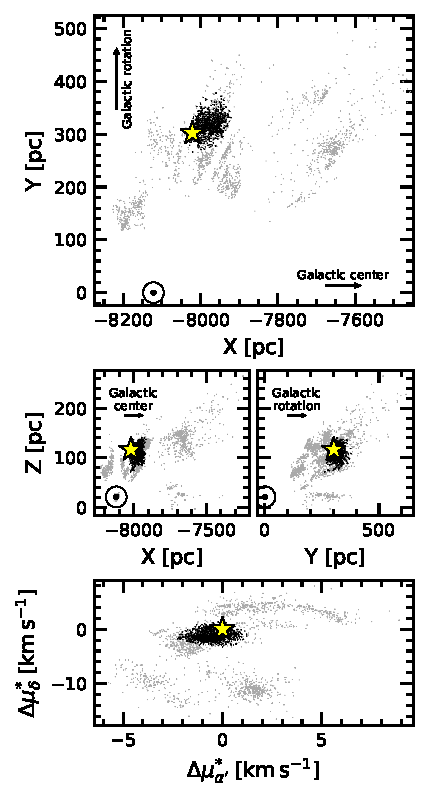
\includegraphics[width=0.47\textwidth]{f1.pdf}
	\end{center}
	\vspace{-0.7cm}
	\caption{
		{\bf Kepler's view of the $\delta$~Lyr cluster.} Each black circle is a
		candidate cluster member, selected from the catalog of \citet{KounkelCovey2019} based on its
		position and kinematics.
		Of the \nkinematic\ candidate cluster members, 58 have at least one
		quarter of Kepler data.  TESS has also observed most of the
		cluster, for one to two lunar months to date.
		\label{fig:skychart}
	}
\end{figure}



\subsection{The Cluster's Age}
\label{sec:clusterage}

\begin{figure*}[tp]
	\begin{center}
		\leavevmode
		\subfloat{
			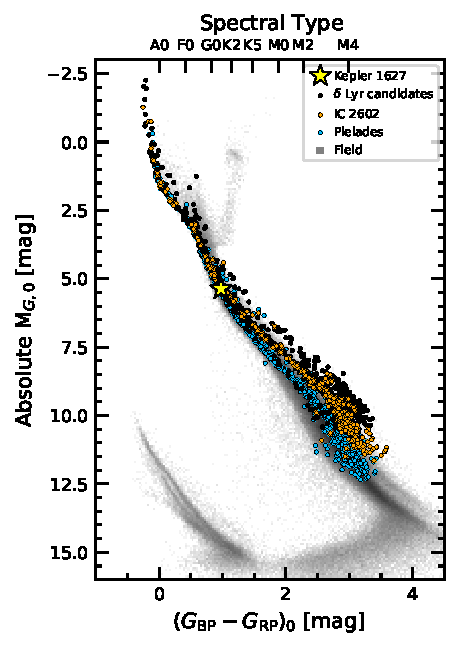
\includegraphics[width=0.49\textwidth]{f2a.pdf}
			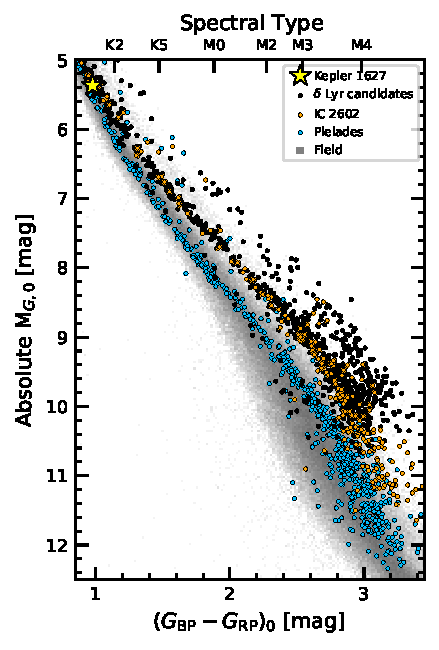
\includegraphics[width=0.469\textwidth]{f2b.pdf}
		}
		
		\vspace{-0.6cm}
		\subfloat{
			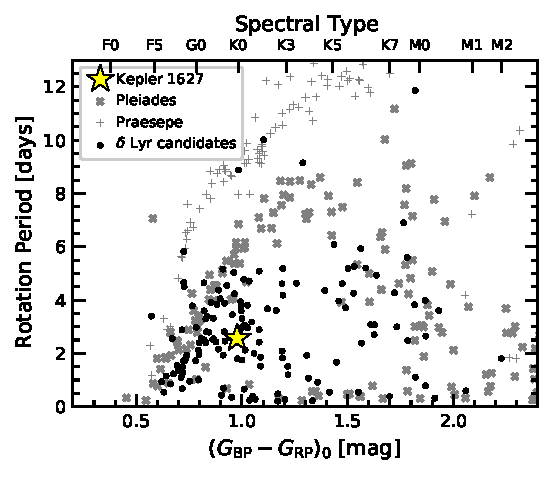
\includegraphics[width=0.7\textwidth]{f2c.pdf}
		}
	\end{center}
	\vspace{-0.7cm}
	\caption{
		{\bf The \cn\ is \clusterage\ old.}  {\it Top:} Color-absolute
		magnitude diagram of candidate \cn\ members, in addition to stars
		in IC\,2602 ($\approx38$\,Myr), the Pleiades ($\approx 115$\,Myr),
		and the Gaia EDR3 Catalog of Nearby Stars (gray background).  The
		zoomed right panel highlights the pre-main-sequence.  The \cn\ and
		IC\,2602 are approximately the same isochronal age.  {\it Bottom:}
		TESS and Kepler stellar rotation period versus dereddened Gaia
		color, with the Pleiades and Praesepe (650\,Myr) shown for
		reference \citep{rebull_rotation_2016a,douglas_poking_2017}.  Most
		candidate \cn\ members are gyrochronally younger than the Pleiades; outliers are
		probably field interlopers.
		\label{fig:age}
	}
\end{figure*}


\subsubsection{Color-Absolute Magnitude Diagram}
\label{sec:camd}

We measured the isochrone age using an empirical approach.  The left
panel of Figure~\ref{fig:age} shows the color-absolute magnitude
diagram (CAMD) of candidate \cn\ members, IC\,2602, the Pleiades, and the
field.  
The stars from the Pleiades and IC\,2602 were adopted from
\citet{cantatgaudin_gaia_2018}, and the field stars are from the Gaia
EDR3 Catalog of Nearby Stars \citep{gaia_gcns_2021}.  We cleaned these
following the data filtering criteria from
\citet[][Appendix B]{GaiaCollaboration2018}, except that we weakened the parallax
precision requirement to $\varpi/\sigma_\varpi>5$.  These filters were
designed to include genuine binaries while omitting instrumental
artifacts.  We then corrected for extinction by querying the
3-dimensional maps of \citet{capitanio_threedimensional_2017} and
\citet{lallement_threedimensional_2018}\footnote{\url{https://stilism.obspm.fr/}, 2021/09/25},
and applied the extinction coefficients $k_X\equiv A_X/A_0$
computed by \citet{GaiaCollaboration2018} assuming that $A_0 = 3.1
E(B-V)$.  For IC\,2602, the Pleiades, and the \cn, this procedure
yielded a respective mean and standard deviation for the reddening of
$E(B-V)=\{0.020\pm0.003, 0.045\pm0.008, 0.032\pm0.006\}$.  These
values agree reasonably well with previously reported values from the
literature \citep[{\it
e.g.},][]{GaiaCollaboration2018,kounkel_untangling_2019,bossini_age_2019}.

% Gaia+2018 E(B-V):
% Pleiades 0.045, IC2602 0.031
%
% Randich+2018 E(B-V):
% Pleiades ??, IC2602 0.032 - 0.092
%
% KC2019: AV->E(B-V)
% Pleiades 0.220 AV -> 0.071
% IC2602 0.243297 -> 0.078
% Stephenson1 0.184 -> 0.059
%
% Bossini+2019 AV->E(B-V)
% PleiadesMelotte22 0.140 -> 0.045
% IC2602 0.096 -> 0.031
% Steph1: 0.157 -> 0.051

Figure~\ref{fig:age} shows that the \cn\ and IC\,2602 overlap, and
therefore are approximately the same age.  In our exploration, we also
compared against $\mu$-Tau ($62\pm7$\,Myr; \citealt{gagne_mutau_2020})
and the Upper-Centaurus-Lupus (UCL) component of the Sco OB2
association ($\approx$$16$\,Myr; \citealt{pecaut_star_2016}).  The
pre-main-sequence M dwarfs of the \cn\ were intermediate between the
latter two clusters.  To turn this heuristic interpolation into an age
measurement, we used the empirical method developed by
\citet{gagne_mutau_2020}.  In brief, we fitted the pre-main-sequence
loci of a set of reference clusters, and the locus of the target \cn\
was then modeled as a piecewise linear combination of these reference
clusters.  For our reference clusters, we adopted members of UCL,
IC\,2602, and the Pleiades from \citet{damiani_stellar_2019} and
\cite{CantatGaudin2018a} respectively.  We removed binaries by
requiring $\texttt{RUWE}<1.3$, $\texttt{radial\_velocity\_error}$
below the 80$^{\rm th}$ percentile of each cluster's distribution, and
manually excluded stars that were obvious photometric binaries in the
CAMD.  We then passed a moving box average and standard deviation
across the CAMD in 0.10\,mag bins, fitted a univariate spline to the
binned values, and assembled a piecewise grid of hybrid isochrones
spanning the ages between UCL to the Pleiades using Equations~6 and~7
from \citet{gagne_mutau_2020}.  

% Randich+18: 43.7 +4.3 - 3.9 LDB, for E(B-V) = 0.068 +/- 0.025
% Dobbie+10: 46 +6 -5 LDB, for 

The ages returned by this procedure depend on the ages assumed for
each reference cluster.  We adopted a 115\,Myr age for the Pleiades \citep{dahm_2015},
and a 16\,Myr age for UCL \citep{pecaut_star_2016}.  The age
of IC\,2602 however is the most important ingredient, since it
receives the most weight in the interpolation.  Plausible ages for
IC\,2602 span 30\,Myr to 46\,Myr, with slightly older ages being
preferred by the lithium-depletion-boundary (LDB) measurements 
\citep{dobbie_ic_2010,randich_gaiaeso_2018}
and
younger ages by the main-sequence turn-off
\citep{stauffer_rotational_1997,david_ages_2015,bossini_age_2019}.
If we were to adopt the 30\,Myr age for IC\,2602, then the \cn\ would
be $31^{+5}_{-4}$\,Myr old.  For the converse extreme of 46\,Myr, the
\cn\ would be $44^{+8}_{-7}$\,Myr old.  We adopt an intermediate
38\,Myr age for IC\,2602, which yields an age for the \cn\ of
\clusterage.\footnote{Our exploration of the PARSEC and MIST isochrone
models over a grid of ages, metallicities, and reddenings, yielded the
best agreement for this $\approx 38\,$Myr age as well, given ${\rm
[Fe/H] = +0.1}$ and $A_V=0.2$
\citep{bressan_parsec_2012,choi_mesa_2016};  this preferred CAMD
reddening is higher than the \citet{lallement_threedimensional_2018}
value by a factor of two.  } Follow-up studies of the LDB or
main-sequence turn-off in the \cn\ could help determine a more precise
and accurate age for the cluster, and are left for future work.





\subsubsection{Stellar Rotation Periods}

Of the \noriginal\ candidate \cn\ members reported by
\citet{kounkel_untangling_2019}, \nwithtess\ stars were amenable to
rotation period measurements ($G<17$ and $\bpmrpo>0.5$) using the TESS
full frame image data.\footnote{Kepler rotation periods were derived
by \citet{mcquillan_rotation_2014} for 28 stars; for these cases, we
adopted the Kepler rotation period.  } We extracted light curves from
the TESS images using the nearest pixel to each star, and regressed
them against systematics with the causal pixel model implemented in
the \texttt{unpopular} package \citep{hattorio_2021_cpm}.  We then
measured candidate rotation periods using a Lomb-Scargle periodogram
\citep{lomb_1976,scargle_studies_1982,astropy_2018}.  To enable cuts
on crowding, we queried the Gaia source catalog for stars within a
$21\farcs0$ radius of the target star (a radius of 1 TESS pixel).
Within this radius, we recorded the number of stars with greater
brightness than the target star, and with brightness within 1.25 and
2.5 TESS magnitudes of the target star.  

We then cleaned the candidate TESS rotation period measurements
through a combination of automated and manual steps.  As a matter of
scope, we restricted our attention to the \nkinwithtess\ stars
discussed in Section~\ref{sec:kinematicselection} in the spatial and
kinematic proximity of Kepler\,1627.  To avoid blending, we also only
focused on stars for which no companions were known with a brightness
exceeding one-tenth of the target star in a $21\farcs0$ radius.  There
were \nkinwithtessandcrowding\ stars that met these requirements, and
that had TESS data available.  For plotting purposes we then imposed a
selection based on the strength of the signal itself: we required the
Lomb Scargle power to exceed 0.2, and the period to be below 15\,days.

The lower panel of Figure~\ref{fig:age} shows the resulting
\nkindefaultcleaning\ stars.  The majority of these stars fall below
the ``slow sequence'' of the Pleiades, consistent with a gyrochronal
age for the \cn\ below 100\,Myr.  In fact, the rotation-color
distributions of other 30\,Myr to 50\,Myr clusters ({\it e.g.},
IC\,2602 and IC\,2391) are indistinguishable
\citep{douglas_stephanie_t_2021_5131306}. 
Approximately 10 of the \cn\ stars appear as outliers above
the ``slow sequence''.  Assuming that they are all false positives
({\it i.e.}, field interlopers), our rotation period detection
fraction would be $\nrotgood/\nkinwithtessandcrowding \approx
\nfracprot\%$.   
The other stars are likely to be field contaminants.
A final possible confounding factor -- binarity -- is known to affect
the density of stars that fall beneath the slow sequence
\citep{meibom_effect_2007,gillen_ngts_2020,bouma_2021_ngc2516}.  We do
not expect it to change the central conclusion regarding the cluster's
age.


\section{The Stars}
\label{sec:stars}

\subsection{Kepler\,1627A}
\subsubsection{Age}
Based on the spatial and kinematic association of \sn\ with the \cn,
and the assumption that the planet formed shortly after the star, it
seems likely that \sn\ is the same age as the cluster. There are
two consistency checks on whether this is true: rotation and lithium.  Based on the Kepler
light curve, the rotation period is $2.642\pm0.042$\,days, where the
quoted uncertainty is based on the scatter in rotation periods
measured from each individual Kepler quarter.  This is consistent with
comparable cluster members (Figure~\ref{fig:age}).

To infer the abundance of Li\,\textsc{I} from the 6708\,\AA\ doublet
\citep[{\it e.g.},][]{soderblom_ages_2014}, we acquired an iodine-free
spectrum from Keck/HIRES on the night of 2021 March 26 using the
standard setup and reduction techniques of the California Planet
Survey \citep{howard_cps_2010}.  Following the equivalent width
measurement procedure described by \citet{bouma_2021_ngc2516}, we find
${\rm EW}_{\rm Li} = 233^{+5}_{-7}$\,m\AA.   This value does not
correct for the Fe\,\textsc{I} blend at 6707.44\AA.  Nonetheless,
given the stellar effective temperature (Table~\ref{tab:starparams}),
this measurement is in agreement with expectations for a
$\approx40$\,Myr star ({\it e.g.}, as measured in IC~2602 by
\citealt{randich_gaiaeso_2018}).  It is also larger than any lithium
equivalent widths measured by \citet{berger_identifying_2018} in their
analysis of 1{,}301 Kepler-star spectra.


\subsubsection{Stellar Properties}

The adopted stellar parameters are listed in
Table~\ref{tab:starparams}.  The stellar mass, radius, and effective
temperature are found by interpolating against a 38$\,$Myr MIST
isochrone \citep{choi_mesa_2016}.  
The statistical uncertainties are propagated from the absolute
magnitude (mostly originating from the the parallax uncertainty) and the color; the systematic
uncertainties are taken to be the difference between the PARSEC
\citep{bressan_parsec_2012} and MIST isochrones.  Reported
uncertainties are a quadrature sum of the statistical and systematic
components.
As a consistency check, 
we analyzed the aforementioned Keck/HIRES spectrum from
the night of 2021 March 26 using a combination of
\texttt{SpecMatch-Emp} for stellar properties, and
\texttt{SpecMatch-Synth} for $v\sin i$
\citep{yee_SM_2017}.
This procedure yielded
$T_{\rm eff}=5498\pm100\,{\rm K}$,
$\log g=4.6\pm0.1$, $[{\rm Fe/H}]=0.15\pm0.10$ 
from \texttt{SpecMatch-Emp}, and $v\sin i = 18.9\pm1.0$ from
\texttt{SpecMatch-Synth}.
These values are within the $1$-$\sigma$ uncertainties of our adopted values from
the isochrone interpolation.


\subsection{Kepler\,1627B}

\begin{figure*}[tp]
	\begin{center}
		\leavevmode
		\subfloat{
			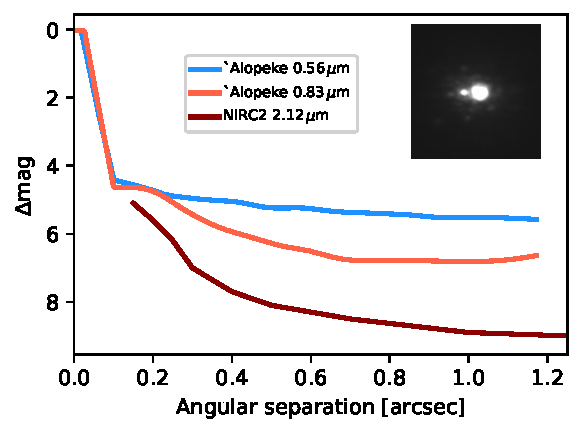
\includegraphics[width=0.49\textwidth]{f10a.pdf}
			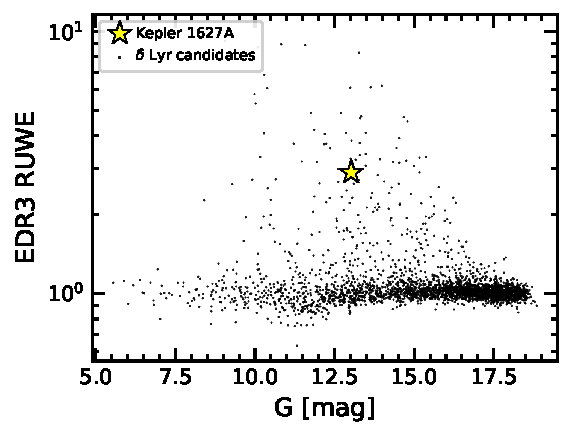
\includegraphics[width=0.48\textwidth]{f10b.pdf}
		}
	\end{center}
	\vspace{-0.5cm}
	\caption{
    {\bf Kepler 1627 is a binary.} {\it Left:} High-resolution imaging
    from Gemini-North/`Alopeke and Keck/NIRC2 shows an $\approx$M2.5V
    companion at $\rho \approx 0\farcs16$, which corresponds to a
    projected separation of $53\pm4$\,AU.  The inset shows a cutout of
    the stacked NIRC2 image (North is up, East is left, scale is set by the
    separation of the binary).  The lines show 5-$\sigma$ contrast
    limits for the `Alopeke filters, and 6-$\sigma$ contrast limits
    for NIRC2 outside of $0\farcs15$. {\it Right:} Gaia
    EDR3 renormalized unit weight error (RUWE) point estimates for
    candidate $\delta$\,Lyr cluster
    members from Figure~\ref{fig:XYZvtang}.  Since other members of the
    cluster with similar brightnesses have comparable degrees of
    photometric variability, the high RUWE independently suggests that Kepler\,1627
    is a binary. 
    \label{fig:kep1627binary}
	}
\end{figure*}

We first noted the presence of a close neighbor in the \sn\ system on 2015 July 22 when
we acquired adaptive optics imaging using the NIRC2 imager on
Keck-II.
We used the narrow camera (FOV = 10.2\arcsec) to obtain 8
images in the $K'$ filter ($\lambda = 2.12\,\mu$m) with a total
exposure time of 160\,s. We analyzed these data following
\citet{kraus_impact_2016}, which entailed using PSF-fitting to measure the separation,
position angle, and contrast of the candidate companion. 
The best-fitting empirical PSF template was identified from among the
near-contemporaneous observations of single stars in the same filter.
The mean values inferred from the 8 images are reported in
Table~\ref{tab:starparams}.
To estimate the detection limits, we analyzed the residuals after subtracting
the empirical PSF template. Within each residual
image, the flux was measured through 40\,mas apertures centered on
every pixel, and then the noise as a function of radius was estimated
from the RMS within concentric rings. Finally, the detection limits
were estimated from the strehl-weighted sum of the detection
significances in the image stack, and we adopted the $6$-$\sigma$
threshold as the detection limit for ruling out additional companions.

We also observed \sn\ on Gemini-North using the `Alopeke speckle
imager on 2021 June 24.  `Alopeke is a dual-channel speckle
interferometer that uses narrow-band filters centered at 0.83\,$\mu$m
and $0.56\,\mu$m.  We acquired three sets of $1000\times 60$$\,$msec
exposures during good seeing (0.45$''$), and used the autocorrelation
function of these images to reconstruct a single image and 5-$\sigma$
detection limits (see \citealt{howell_speckle_2011}).  This procedure
yielded a detection of the companion in the 0.83\,$\mu$m notch filter,
but not the $0.56\,\mu$m filter.  The measured projected separation
and magnitude difference are given in Table~\ref{tab:starparams}.

Figure~\ref{fig:kep1627binary} summarizes the results of the
high-resolution imaging.  The Gaia EDR3 parallax for the primary
implies a projected separation of $53 \pm 4$\,AU, assuming the
companion is bound.  Although the companion is unresolved in the Gaia
source catalog (there are no comoving, codistant candidate companions
brighter than $G < 20.5$ mag within $\rho < 120\arcsec$), its
existence was also suggested by the primary star's large renormalized unit weight error (RUWE),
relative to other members of the \cn.  Based on the apparent
separation, the binary orbital period is of order hundreds of years.
The large RUWE is therefore more likely to be caused by a PSF-mismatch
skewing the Gaia centroiding during successive scans, rather than true
astrometric motion.  Regardless, given the low geometric probability that a companion imaged at
$\rho \approx 0\farcs16$ is a chance line-of-sight companion, we
proceed under the assumption that the companion is bound, and that
Kepler\,1627 is a binary.  
Given the distance and age, the models of
\citet{baraffe_new_2015} imply a companion mass of $M_{\rm B} \approx
0.33 M_{\odot}$ and companion temperature of $T_{\rm eff,B} \approx
3450$ K.  The corresponding spectral type is roughly M2.5V
\citep{pecaut_mamajek_2013}.
% \footnote{\url{http://www.pas.rochester.edu/~emamajek/EEM_dwarf_UBVIJHK_colors_Teff.txt}, version \texttt{2021/03/02}.}
These models combined with the NIRC2 contrast limits similarly imply
physical limits on tertiary companions of $M_{\rm ter} < 50
M_{\rm Jup}$ at $\rho = 50$\,AU, $M_{\rm ter} < 20 M_{\rm Jup}$ at $\rho =
100$\,AU, and $M_{\rm ter} < 10 M_{\rm Jup}$ at $\rho = 330$\,AU.



\section{The Planet}
\label{sec:planet}

\begin{figure*}[tp]
	\begin{center}
		\leavevmode
		\subfloat{
			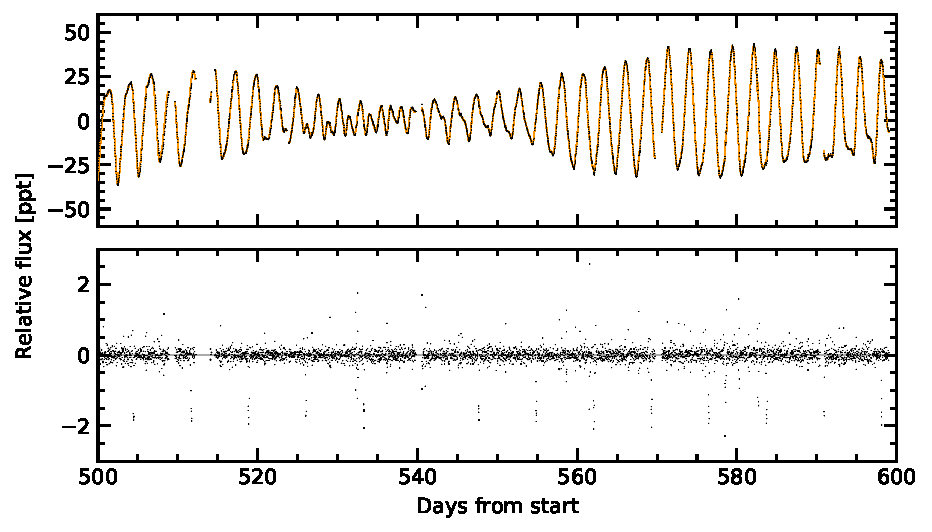
\includegraphics[width=\textwidth]{f3a.pdf}
		}

		\vspace{-0.2cm}	
		\subfloat{
			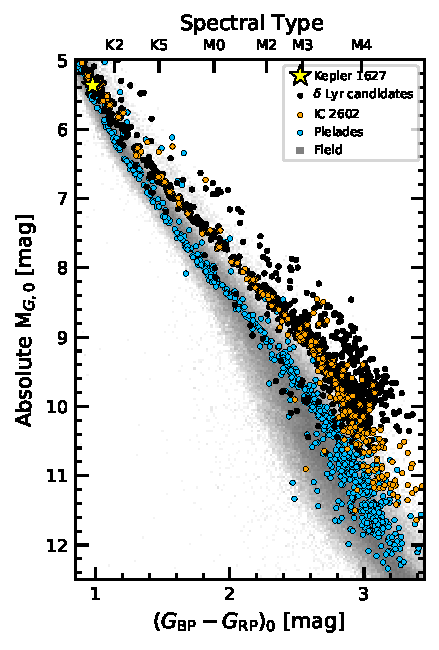
\includegraphics[width=0.5\textwidth]{f3b.pdf}
			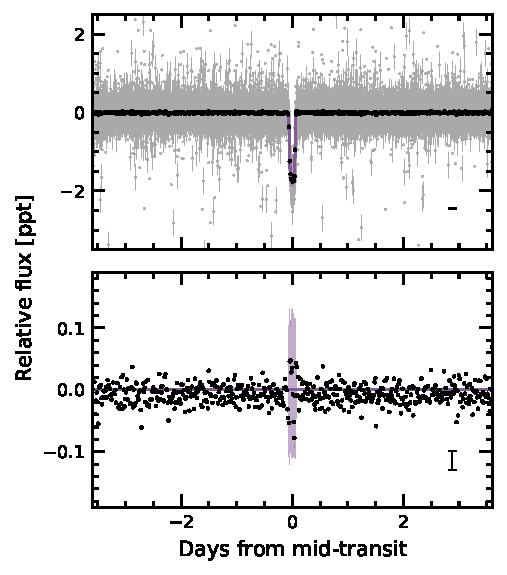
\includegraphics[width=0.5\textwidth]{f3c.pdf}
		}
	\end{center}
	\vspace{-0.7cm}
  \caption{ {\bf The light curve of Kepler\,1627.}
    {\it Top}: 
    The Kepler data span 1{,}437 days (3.9 years), sampled at
    30 minute cadence;  a 100 day segment is shown.  The
    top panel shows the \texttt{PDCSAP} median-subtracted flux in
    units of parts-per-thousand ($\times 10^{-3}$).  The dominant
    signal is induced by starspots.  The stellar
    variability model (orange line) is subtracted below, revealing the
    transits of \pn.  The
    online Figure Set spans the entire 3.9 years of observations.
    {\it Bottom}:
    Phase-folded transit of Kepler 1627Ab with stellar variability
    removed.  Windows over 20 hours ({\it left}) and the entire orbit
    ({\it right}) are shown, and the residual after subtracting the
    transit is in the bottom-most row.  The 2-$\sigma$ model uncertainties
    and the best-fit model are the light purple band and the dark
    purple line.  Gray points are individual flux measurements; black
    points bin these to 20 minute intervals, and have a representative
    1-$\sigma$ error bar in the lower right of each panel.  The asymmetric
    residual during transit is significantly larger than the out-of-transit scatter.
    \label{fig:lc}
  }
\end{figure*}

\subsection{Kepler Light Curve}

The Kepler space telescope observed \sn\ at a 30-minute cadence from
2009 May 2 until 2013 April 8.  Data gaps during quarters 4, 9, and 13
led to an average duty cycle over the 3.9~year interval of 78\%.  \sn\
was also observed at 1-minute cadence from 2012 Oct 5 until 2013 Jan
11.  The top panel of Figure~\ref{fig:lc} shows a portion of the 30-minute
cadence \texttt{PDCSAP} light curve.  Nonastrophysical variability has
been removed using the methods discussed by
\citet{smith_kepler_PDC_2017}; the default optimal aperture was
assumed \citep{smith_finding_2016}. 
Cadences with non-zero quality flags (9\% of the data) have been omitted.
 The resulting photometry is dominated by
a quasi-periodic starspot signal with a peak-to-peak amplitude that
varies between 2\% and 8\%.  
Previous analyses have identified and
characterized the hidden transit signal
\citep{2012ApJS..199...24T,thompson_planetary_2018}, validated its
planetary nature \citep{morton_false_2016}, and even searched the
system for transit timing variations \citep{holczer_transit_2016}.
Nonetheless, since the cluster membership provides us
with more precise stellar parameters than those previously available,
we opted to reanalyze the
light curve.

We fitted the Kepler long cadence time series with a model that
simultaneously included the planetary transit and the stellar
variability.  The stellar variability was modeled with the
\texttt{RotationTerm} Gaussian Process kernel in \texttt{exoplanet}
\citep{exoplanet:exoplanet}.  This kernel assumes that the variability
is generated by a mixture of two damped simple harmonic oscillators
with characteristic frequencies set by 1/$P_{\rm rot}$ and its first
harmonic.  We additionally included a jitter term to inflate
the flux uncertainties in a manner that accounted for otherwise
unmodeled excess white noise, and let the eccentricity float.  For
the limb-darkening, we assumed a quadratic law, and sampled using the
uninformative prior suggested by \citet{exoplanet:kipping13}.

Our model therefore included 10 free parameters for the transit ($\{P,
t_0, R_{\rm p}/R_\star, b, u_1 ,u_2 ,R_\star, \log g, e, \omega \}$),
2 free parameters for the light curve normalization and a white noise 
jitter ($\{\langle f \rangle, \sigma_f \}$), and 5
hyperparameters for the GP ($\{\sigma_{\mathrm{rot}},
P_{\mathrm{rot}}, Q_0, \mathrm{d}Q, f \}$).  We also considered
including an additive \texttt{SHOTerm} kernel to account for
stochastic noise, but found that this did not significantly affect the
results, and so opted for the simpler GP kernel.  We fitted the models
using \texttt{PyMC3} \citep{salvatier_2016_PyMC3,exoplanet:theano},
and accounted for the finite integration time of each exposure in the
numerical integration when evaluating the model light curve
\citep[see][]{kipping_binning_2010}.  We assumed a Gaussian
likelihood, and after initializing each model with the parameters of
the maximum {\it a posteriori} model, we sampled using
\texttt{PyMC3}'s gradient-based No-U-Turn Sampler
\citep{hoffman_no-u-turn_2014} in the bases indicated in
Table~\ref{tab:posterior}.  We used $\hat{R}$ as our convergence
diagnostic \citep{gelman_inference_1992}.

Figure~\ref{fig:lc} shows the resulting best-fit model in orange (top) and
purple (bottom).
The model parameters and their uncertainties, given in Table~\ref{tab:posterior}, are
broadly consistent with a mini-Neptune sized planet ($3.36\pm0.18\,R_\oplus$) on a close-in circular\footnote{ Our transit fitting
	yields $e<0.48$ at 2-$\sigma$; the constraints on the eccentricity are
	not particularly strong.} orbit around a G8V host star ($0.88 \pm 0.02
R_\odot$).  Our best-fit planet size is smaller than that
previously reported by \citet{morton_false_2016} and
\citet{berger_identifying_2018}, at 0.7-$\sigma$ and 1.2-$\sigma$
confidence respectively.  The former is explained by differing
assumptions about the stellar radius; the latter appears to be due to
differences in the measured transit depth, which could be linked to
the different methods used to account for the stellar rotation signal.

The transit fit however is not perfect: the lower panels of
Figure~\ref{fig:lc} show an asymmetric
residual in the data relative to the model: the measured flux is systematically
high during the first half of transit, and low in the second half.  The
semi-amplitude of this deviation is $\approx50\,{\rm ppm}$, which
represents a $\approx 3\%$ distortion of the transit depth
($\approx1700\,{\rm ppm}$).  
Note that
while this asymmetry is within the 2-$\sigma$ model
uncertainties, the model has a jitter term that grows to
account for otherwise unmodeled white noise in the flux.  The
significance of the asymmetry is therefore best assessed in comparison
against the intrinsic out-of-transit scatter in the data, not the model
uncertainties.

To determine whether the asymmetry is a systematic caused by our stellar variability model,
we explored an alternative
approach in which we isolated each transit window and locally fitted
out polynomial trends, and then binned all the observed transits; the
asymmetry was still present at a comparable amplitude.  
Appendix~\ref{app:asymmetry} includes a deeper analysis, and
finds that the asymmetry also seems to be robust to different methods of
data binning.  Plausible astrophysical explanations are given in
Section~\ref{sec:conc}.


\subsection{Planet Confirmation}


\begin{figure}[tp]
	\begin{center}
		\leavevmode
		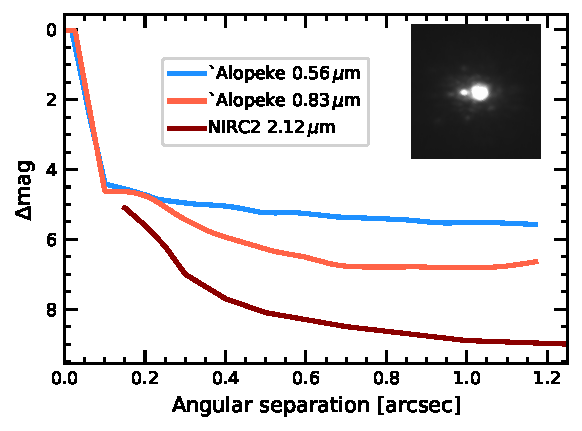
\includegraphics[width=0.47\textwidth]{f4a.pdf}
	\end{center}
	\vspace{-0.7cm}
	\caption{
		{\bf Evidence for a prograde orbit of Kepler 1627 Ab.}
		The time of each Kepler transit was measured, along with the local
		slope of the light curve.  The two quantities appear
		anti-correlated, which is most easily explained by starspot
		crossings during the first (second) half of transit inducing a
		positive (negative) TTV, provided that the orbit is prograde
		\citep{mazeh_time_2015}.  The units along the abscissa are most
		easily understood by considering that the stellar flux changes by
		$\sim$60\,ppt per half rotation period ($\sim$1.3\,days).
		\label{fig:corr}
	}
\end{figure}

% rotation period from plot_rotation_period_windowslider.py

If the \pn\ transit signal is created by a genuine planet,  then to
our knowledge it would be the youngest planet yet found by the main
Kepler mission.\footnote{The re-purposed K2 mission however has found
two younger systems containing five planets: K2-33b ($9\pm1\,{\rm
Myr}$; \citealt{Mann_K2_33b_2016,David_et_al_2017}) and V1298 Tau
($23\pm4\,{\rm Myr}$; \citealt{david_four_2019}).}   
Could the transit be produced by anything other than a planet
orbiting this near-solar analog?  \citet{morton_false_2016} validated
the planet based on the transit shape, arguing that the most probable
false positive scenario was that of a background eclipsing binary,
which had a model-dependent probability of $\approx10^{-5}$.  However,
this calculation was performed without knowledge of the low-mass stellar companion ($M_{\rm B}\approx
0.33\,M_\odot$).  
Validated planets have also previously been refuted \citep[{\it e.g.},][]{shporer_three_2017}.
We therefore reassessed
false positive scenarios in some detail. 

% (0.7-2.0\% V-band to G-band dmag difference from EEM table; NOTE
% could determine using model spectra)
As an initial plausibility check,
Kepler\,1627B contributes 1\% to 2\% of the total flux observed in
the Kepler aperture.  
For the sake of argument, assume the former value.
The observed transit has a depth of $\approx$0.17\%.  A
17\% deep eclipse of the secondary star would therefore be needed to
produce a signal with the appropriate depth.  The shape of the
transit signal however requires the impact parameter to be below 0.74
(Table~\ref{tab:posterior}); the tertiary transiting the secondary would
therefore need to be non-grazing with $R_3/R_2 \approx 0.4$.
%Assuming a $\approx 0.46R_\odot$ radius of the imaged secondary
%from the \citet{baraffe_new_2015} models, this
%would imply a tertiary stellar radius of $\approx 0.2R_\odot$.
This
yields a contradiction:  this scenario would require an ingress and
egress phase that each span $\approx$40\% of the transit duration
($\approx 65\,{\rm minutes}$).  The actual measured ingress and egress
duration is $\approx 15\,{\rm minutes}$, 4.4$\times$ shorter.  The
combination of Kepler 1627B's brightness, the transit depth, and the ingress
duration therefore disfavor the scenario that Kepler 1627B might host the
transit signal.  

% Baraffe+15: M_B 0.33 Mdot
% Rstar = 0.455 --> 0.465 Rsun
% 

% At 30 Myr, a 0.44\,$M_\odot$ solar-metallicity dwarf is $\approx 26\%$
% larger than when it is fully contracted on the main sequence
% (0.40\,$R_\odot$ vs{.} 0.50\,$R_\odot$; ).

There are two other new lines of evidence that confirm the planetary
interpretation.  First, the transit duration and the orbital period
are inconsistent with an eclipsing body around the M-dwarf companion:
we find $\rho_\star = 2.00 \pm 0.24\,{\rm g\,cm}^{-3}$, while the
theoretically expected density for the companion is $\approx 4.6\,{\rm
g\,cm}^{-3}$ (Table~\ref{tab:posterior}; \citealt{choi_mesa_2016}).
The transit duration is therefore too long to be explained by a star
eclipsing the M dwarf secondary at $10$-$\sigma$.

%NOTE to the arxiv readers:, the $\approx$100 days of short-cadence
%Kepler observations also mitigate the cadence-induced smearing, and
%enable a more precise measurement of the transit impact parameter
%\citep{kipping_binning_2010}.  The planet transits with $b<0.YY$
%(2-$\sigma$) from the 1-minute data, compared to $<0.76$ (2-$\sigma$)
%from the 30-minute data.  This implies an even stronger constraint on
%the transit shape in an analysis of the false positive probability.

The second line of confirming evidence comes by analyzing the
individual Kepler transit times. We isolated each of the 144 observed
transits to within $\pm4.5$\,hr of each transit, and fitted each
window with both {\it i)} a local second-order polynomial and transit,
and {\it ii)} a local linear trend.  We let the mid-time of each
transit float, and then calculated the residual between the measured
mid-time and that of a periodic orbit.  This residual, the transit
timing variation (TTV), is plotted in Figure~\ref{fig:corr}
against the local linear slope.  A significant correlation of $-0.0564
\pm 0.0098\ {\rm ppt\,day}^{-1}$ is observed.  Fewer than ten Kepler
Objects of Interest have shown this correlation
\citep{holczer_time_2015}, which is most readily interpreted as a TTV
induced by unresolved starspot crossings \citep{mazeh_time_2015}.
This is only possible if the planet transits the primary star, which
excludes a background eclipsing binary scenario, and therefore
confirms that \pn\ is a planet.  It also suggests that the planet's
orbit is prograde.  The latter point assumes that the dominant
photometric variability is induced by dark spots, and not bright
faculae.  Given the observed transition of Sun-like stellar
variability from spot to faculae-dominated regimes between young and
old ages, we expect this assumption to be reasonably secure
\citep{shapiro_are_2016,montet_long-term_2017,reinhold_stellar_2020}.


\begin{figure}[t]
	\begin{center}
		\leavevmode
		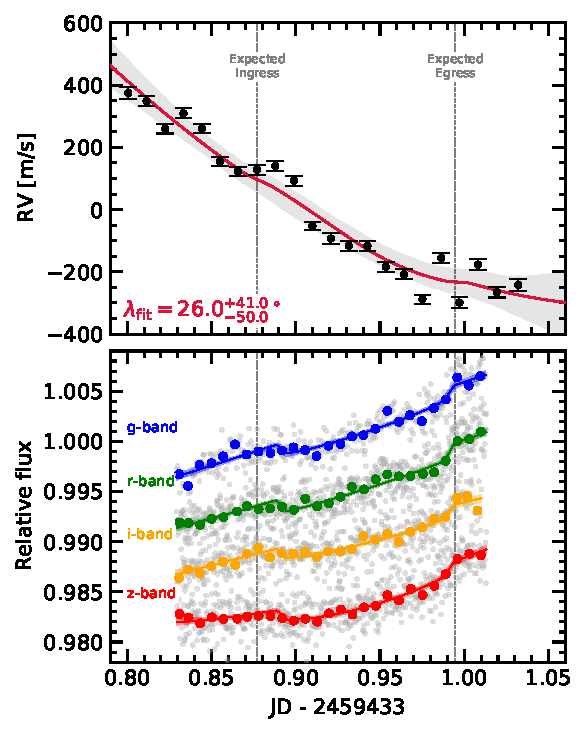
\includegraphics[width=0.47\textwidth]{f4b.pdf}
	\end{center}
	\vspace{-0.7cm}
	\caption{
		{\bf Radial velocities acquired using Keck/HIRES during the transit of
			2021 Aug 7, observed simultaneously with MuSCAT3.}  Shaded bands
		show 2-$\sigma$ model uncertainties.  The photometric transit
		depths are consistent across the {\it griz} bandpasses.  The
		best-fitting model in the top panel includes the RM effect and a quadratic trend
		in time.  The radial velocity scatter
		between exposures ($\sigma_{\rm RV}\approx50$\ms) prevented us from detecting the RM
		effect.
		\label{fig:ground}
	}
\end{figure}

A third supporting line of evidence for the planetary interpretation
exists, though we consider it less definitive than the stellar
density and TTV-local slope correlation.  We observed a transit of
\pn\ on the night of 2021 Aug 7 simultaneously with Keck/HIRES and
MuSCAT3.  We scheduled the observations using the ephemeris of
\citet{holczer_transit_2016}.  Although we did not detect the
Rossiter-McLaughlin (RM) anomaly, the multi-band MuSCAT3 light curves
show the transit (Figure~\ref{fig:ground}).  Fitting
the MuSCAT3 photometry with a model that lets the transit depths vary
across each bandpass, we find {\it griz} depths consistent with the
Kepler depth at 0.6, 0.3, 0.3, and 1.1-$\sigma$ respectively.  The
MuSCAT3 observations also suggest a transit duration $17.4\pm3.6\ {\rm
minutes}$ shorter than the Kepler transits; further photometric
follow-up could help confirm whether the transit duration is indeed
changing.  For our RM analysis, the details are discussed in
Appendix~\ref{app:rm}.  While the velocities are marginally more
consistent with a prograde or polar orbit than a retrograde orbit, the
spot-corrected exposure-to-exposure scatter ($\sigma_{\rm RV}\approx
50$\ms) is larger than the expected velocity anomaly
($\Delta v_{\rm RM}\approx 20\,{\rm m\,s}^{-1}$).  We are therefore
not in a position to claim a spectroscopic detection of the RM effect,
nor to quantify the stellar obliquity.


\section{Discussion \& Conclusions}
\label{sec:conc}

\begin{figure*}[tp]
	\begin{center}
		\leavevmode
		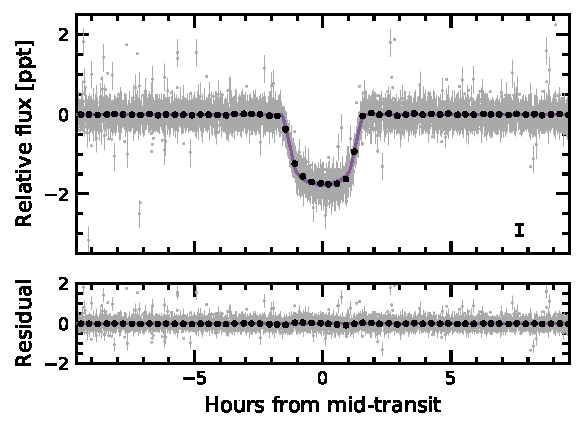
\includegraphics[width=0.7\textwidth]{f5.pdf}
	\end{center}
	\vspace{-0.7cm}
	\caption{
		{\bf Radii, orbital periods, and ages of transiting exoplanets}.
		Planets younger than a gigayear with ${\rm \tau}/\sigma_{\tau} >
		3$ are emphasized, where $\tau$ is the age and $\sigma_{\tau}$ is
		its uncertainty.  \pn\ is shown with a star.  The large sizes of
		the youngest transiting planets could be explained by their
		primordial atmospheres not yet having evaporated; direct
		measurements of the atmospheric outflows or planetary masses would
		help to confirm this expectation.  Selection effects may also be
		important.  Parameters are from the NASA Exoplanet Archive (2021
		Sept 15).
		\label{fig:rp_period_age}
	}
\end{figure*}


Kepler\,1627Ab provides a new extremum in the ages of the Kepler
planets, and opens multiple avenues for further study.  
Observations of spectroscopic transits at greater precision should yield a
measurement of the stellar obliquity, which would confirm or refute the prograde orbital
geometry suggested by the TTV-local slope correlation.  Separately,
transit spectroscopy aimed at detecting atmospheric outflows might
yield insight into the evolutionary state of the atmosphere
\citep[{\it
e.g.},][]{ehrenreich_giant_2015,spake_helium_2018,vissapragada_2020}.
Observations aimed at quantifying the amount of high-energy
irradiation incident on the planet would complement these efforts, by
helping to clarify the expected outflow rate \citep[{\it
e.g.},][]{poppenhaeger_2021}.  Finally, a challenging but informative
quantity to measure would be the planet's mass.  The most feasible
approach would likely be
long-term monitoring of the transit times and durations,
given the technical difficulty of performing a high-cadence multi-color radial velocity campaign
on a $V=13.1$ target.
Measured at sufficient precision though, the mass, combined with the known
age and size, would yield constraints on both the planet's composition
and its initial entropy \citep{owen_constraining_2020}.

More immediately, the Kepler data may yet contain additional
information.  For instance, one possible explanation for the transit
asymmetry shown in Figure~\ref{fig:lc} is that of a dusty asymmetric
outflow.  
A second possibility is that the planetary orbit is slightly misaligned
from the stellar spin axis, and tends to
transit starspot groups at
favored stellar latitudes.
Other possibilities such as gravity darkening or TTVs causing
the asymmetry are disfavored
(see Appendix~\ref{app:asymmetry}).  Dusty outflows are theoretically
expected for young mini-Neptunes, and the amplitude of the observed
asymmetry is also roughly consistent with predictions
\citep{wang_dai_2019}.  Beyond the asymmetric transits,
Appendix~\ref{app:flare} highlights an additional abnormality in the Kepler
data, in the arrival time distribution of stellar flares.  We
encourage its exploration by investigators more versed in the topic
than ourselves.

In the context of the transiting planet population, \pn\ is among the
youngest known (Figure~\ref{fig:rp_period_age}).  Comparable systems
with precise ages include K2-33
\citep{Mann_K2_33b_2016,David_et_al_2017}, DS~Tuc
\citep{benatti_possibly_2019,newton_tess_2019} , HIP~67522
\citep{rizzuto_tess_2020}, TOI~837
\citep{bouma_cluster_2020}, the two-planet AU~Mic system
\citep{plavchan_planet_2020,martioli_aumicbc_2021} and the four-planet
V1298~Tau system \citep{david_four_2019}.  \pn\ is one of the smallest
planets in this sample ($3.36\pm0.18\,R_\oplus$), which could be linked to the selection effects
imposed by the spot-induced photometric variability at very young ages
\citep[{\it e.g.},][]{zhou_2021_tois}.  If these young
planets have masses between $\approx$5$\,M_\oplus$ and 10$\,M_\oplus$,
then their low densities would be in accord with
the expectation that mini-Neptunes start their lives with large
primordial atmospheres that are shed over the first gigayear
\citep{Owen_Wu_2013,Fulton_et_al_2017,ginzburg_corepowered_2018}.  The
prograde orbit, if confirmed, would be consistent with a quiescent
disk-driven migration history, and would differ from misalignments that
have been observed for some older
hot Neptunes~\citep{sanchis-ojeda_starspots_2011,albrecht_obliquities_2012,dalal_2019_hd3167,rubenzahl_tess-keck_2021}.
%Spectroscopic follow-up observations of the transit remain necessary
%however to verify whether the TTV-slope correlation is yielding the
%correct orbital geometry.

%NB to arxiv readers: The alternative scenario of in-situ formation is
%disfavored on theoretical grounds: the required disk mass would
%likely drive migration, and so lacks internal consistency
%\citep{inamdar_formation_2015,ogihara_reassessment_2015}.

Ultimately, the main advance of this work is a precise measurement of
the age of \pn.   This measurement was enabled by identifying the
connection of the star to the \cn\ using Gaia kinematics, and then by
using the Gaia color-absolute magnitude diagram and TESS stellar rotation periods to verify
the cluster's existence.  Table~\ref{tab:v06} enables similar
cross-matches for both known and forthcoming exoplanet
systems \citep[{\it e.g.},][]{guerrero_tess_2021}.  The entry shown in
the header, HD 150706b, is one example: the
host star appears to be a member of the Ursa Major moving group
($400\,{\rm Myr}$; \citealt{mann_tess_2020}).  Confirming
this suggested kinematic association with independent age indicators is
essential because the false positive rates are not known.
Alternatively, one could instead opt to identify new kinematic
associations around known exoplanet host stars using positions and
tangential velocities from Gaia, and to then verify these associations
with stellar rotation periods and spectroscopy \citep[{\it
e.g.},][]{tofflemire_tess_2021}.  
Each path seems likely to expand the census of planets with precisely
measured ages over the coming years.


%%%%%%%%%%%%%%%%%%%%%%%%%%%%%%%%%%%%%%%%%%%%%%%%%%%%%%%%%%%%%%%%%%%%%%%%%%%%%%%


\clearpage
\acknowledgements
\raggedbottom

The authors are grateful to J{.}~Winn, J{.}~Spake, A{.}~Howard, and
T{.}~David for illuminating discussions and suggestions, and to
R{.}~Kerr for kindly providing us with the \citet{Kerr2021} membership
list prior to its publication.
The authors are also grateful to K{.}~Collins for helping resolve the
scheduling conflict that would have otherwise prevented the MuSCAT3
observations.
% is grateful to G.~Zhou, B{.}~Tofflemire, A{.}~McWilliam,
% E{.}~Newton, M{.}~Kounkel, A{.}~Kraus, L{.}~Hillenbrand, and
% K{.}~Hawkins for the discussions on young stars, rotation, and lithium
% that encouraged this analysis.
%
L.G.B{.} acknowledges support from a Charlotte Elizabeth Procter
Fellowship from Princeton University, as well as from the TESS GI
Program, programs G011103 and G022117, through NASA grants
80NSSC19K0386 and 80NSSC19K1728.
%
%
Keck/NIRC2 imaging was acquired by program 2015A/N301N2L
(PI: A.~Kraus). % and 2019A/N069 (PI: E.~Petigura).
%
In addition, this paper is based in part on observations made with the
MuSCAT3 instrument, developed by the Astrobiology Center and under
financial support by JSPS KAKENHI (JP18H05439) and JST PRESTO
(JPMJPR1775), at Faulkes Telescope North on Maui, HI, operated by the
Las Cumbres Observatory.
%
This work is partly supported by JSPS KAKENHI Grant Numbers 22000005,
JP15H02063, JP17H04574, JP18H05439, JP18H05442, JST PRESTO Grant
Number JPMJPR1775, the Astrobiology Center of National Institutes of
Natural Sciences (NINS) (Grant Number AB031010).
%
% ACKNOWLEDGE PFS / CAMPANAS.
%
This paper also includes data collected by the TESS mission, which are
publicly available from the Mikulski Archive for Space Telescopes
(MAST).
%
Funding for the TESS mission is provided by NASA's Science Mission
directorate.
%
We thank the TESS Architects (G.~Ricker, R.~Vanderspek, D.~Latham,
S.~Seager, J.~Jenkins) and the many TESS team members for their
efforts to make the mission a continued success.
%
%
%This study was based in part on observations at Cerro Tololo
%Inter-American Observatory at NSF's NOIRLab (NOIRLab Prop{.} ID
%2020A-0146; 2020B-0029 PI: Bouma), which is managed by the
%Association of Universities for Research in Astronomy (AURA) under a
%cooperative agreement with the National Science Foundation.
%
%
Finally, this research has made use of the Keck Observatory Archive (KOA),
which is operated by the W. M. Keck Observatory and the NASA Exoplanet
Science Institute (NExScI), under contract with the National
Aeronautics and Space Administration.  We also thank the Keck
Observatory staff for their support of HIRES and remote observing.  We
recognize the importance that the summit of Maunakea has within the
indigenous Hawaiian community, and are deeply grateful to have the
opportunity to conduct observations from this mountain.
%
% The Digitized Sky Survey was produced at the Space Telescope Science
% Institute under U.S. Government grant NAG W-2166.
% Figure~\ref{fig:scene} is based on photographic data obtained using
% the Oschin Schmidt Telescope on Palomar Mountain.
%

% %
% This research made use of the NASA Exoplanet Archive, which is
% operated by the California Institute of Technology, under contract
% with the National Aeronautics and Space Administration under the
% Exoplanet Exploration Program.
% %

% Resources supporting this work were provided by the NASA High-End
% Computing (HEC) Program through the NASA Advanced Supercomputing (NAS)
% Division at Ames Research Center for the production of the SPOC data
% products.
%

% A.J.\ and R.B.\ acknowledge support from project IC120009 ``Millennium
% Institute of Astrophysics (MAS)'' of the Millenium Science Initiative,
% Chilean Ministry of Economy. A.J.\ acknowledges additional support
% from FONDECYT project 1171208.  J.I.V\ acknowledges support from
% CONICYT-PFCHA/Doctorado Nacional-21191829.  R.B.\ acknowledges support
% from FONDECYT Post-doctoral Fellowship Project 3180246.
% %
% C.T.\ and C.B\ acknowledge support from Australian Research Council
% grants LE150100087, LE160100014, LE180100165, DP170103491 and
% DP190103688.
% %
% C.Z.\ is supported by a Dunlap Fellowship at the Dunlap Institute for
% Astronomy \& Astrophysics, funded through an endowment established by
% the Dunlap family and the University of Toronto.
% %
% D.D.\ acknowledges support through the TESS Guest Investigator Program
% Grant 80NSSC19K1727.
%
%
%
% %
% Based on observations obtained at the Gemini Observatory, which is
% operated by the Association of Universities for Research in Astronomy,
% Inc., under a cooperative agreement with the NSF on behalf of the
% Gemini partnership: the National Science Foundation (United States),
% National Research Council (Canada), CONICYT (Chile), Ministerio de
% Ciencia, Tecnolog\'{i}a e Innovaci\'{o}n Productiva (Argentina),
% Minist\'{e}rio da Ci\^{e}ncia, Tecnologia e Inova\c{c}\~{a}o (Brazil),
% and Korea Astronomy and Space Science Institute (Republic of Korea).
% %
% Observations in the paper made use of the High-Resolution Imaging
% instrument Zorro at Gemini-South. Zorro was funded by the NASA
% Exoplanet Exploration Program and built at the NASA Ames Research
% Center by Steve B. Howell, Nic Scott, Elliott P. Horch, and Emmett
% Quigley.
% %
% This research has made use of the VizieR catalogue access tool, CDS,
% Strasbourg, France. The original description of the VizieR service was
% published in A\&AS 143, 23.
% %
% This work has made use of data from the European Space Agency (ESA)
% mission {\it Gaia} (\url{https://www.cosmos.esa.int/gaia}), processed
% by the {\it Gaia} Data Processing and Analysis Consortium (DPAC,
% \url{https://www.cosmos.esa.int/web/gaia/dpac/consortium}). Funding
% for the DPAC has been provided by national institutions, in particular
% the institutions participating in the {\it Gaia} Multilateral
% Agreement.
%
% (Some of) The data presented herein were obtained at the W. M. Keck
% Observatory, which is operated as a scientific partnership among the
% California Institute of Technology, the University of California and
% the National Aeronautics and Space Administration. The Observatory was
% made possible by the generous financial support of the W. M. Keck
% Foundation.
% The authors wish to recognize and acknowledge the very significant
% cultural role and reverence that the summit of Maunakea has always had
% within the indigenous Hawaiian community.  We are most fortunate to
% have the opportunity to conduct observations from this mountain.
%
% \newline
%

\software{
  %\texttt{arviz} \citep{arviz_2019},
  \texttt{altaipony} \citep{ilin_flares_2021},
  \texttt{astrobase} \citep{bhatti_astrobase_2018},
  %\texttt{astroplan} \citep{astroplan2018},
	%\texttt{AstroImageJ} \citep{collins_astroimagej_2017},
  \texttt{astropy} \citep{astropy_2018},
  \texttt{astroquery} \citep{astroquery_2018},
  %\texttt{BATMAN} \citep{kreidberg_batman_2015},
  %\texttt{ceres} \citep{brahm_2017_ceres},
  %\texttt{cdips-pipeline} \citep{bhatti_cdips-pipeline_2019},
  \texttt{corner} \citep{corner_2016},
  %\texttt{emcee} \citep{foreman-mackey_emcee_2013},
  \texttt{exoplanet} \citep{exoplanet:exoplanet}, and its
  dependencies \citep{exoplanet:agol20, exoplanet:kipping13, exoplanet:luger18,
   	exoplanet:theano},
	%\texttt{gala} \citep{gala,PriceWhelan_2017_gala_zenodo},
	%\texttt{IDL Astronomy User's Library} \citep{landsman_1995},
  %\texttt{IPython} \citep{perez_2007},
	%\texttt{isochrones} \citep{morton_2015_isochrones},
	%\texttt{lightkurve} \citep{lightkurve_2018},
  %\texttt{matplotlib} \citep{hunter_matplotlib_2007}, 
  %\texttt{MESA} \citep{paxton_modules_2011,paxton_modules_2013,paxton_modules_2015}
  %\texttt{numpy} \citep{walt_numpy_2011}, 
  %\texttt{pandas} \citep{mckinney-proc-scipy-2010},
  %\texttt{pyGAM} \citep{serven_pygam_2018_1476122},
  \texttt{PyMC3} \citep{salvatier_2016_PyMC3},
  %\texttt{radvel} \citep{fulton_radvel_2018},
  %\texttt{scikit-learn} \citep{scikit-learn},
  \texttt{scipy} \citep{jones_scipy_2001},
  \texttt{TESS-point}  \citep{burke_2020},
  %\texttt{tesscut} \citep{brasseur_astrocut_2019},
	%\texttt{VESPA} \citep{morton_efficient_2012,vespa_2015},
  %\texttt{webplotdigitzer} \citep{rohatgi_2019},
  \texttt{wotan} \citep{hippke_wotan_2019}.
}
\ 

\facilities{
 	{\it Astrometry}:
 	Gaia \citep{gaia_collaboration_gaia_2018,gaia_collaboration_2021_edr3}.
 	{\it Imaging}:
    Second Generation Digitized Sky Survey. %,
    %SOAR~(HRCam; \citealt{tokovinin_ten_2018}).
 	Keck:II~(NIRC2; \url{www2.keck.hawaii.edu/inst/nirc2}).
 	%Gemini:South~(Zorro; \citealt{scott_nessi_2018}.
 	Gemini:North~(`Alopeke; \citealt{scott_nessi_2018,scott_twin_2021}.
 	{\it Spectroscopy}:
	%CTIO1.5$\,$m~(CHIRON; \citealt{tokovinin_chironfiber_2013}),
  %PFS ({\bf CITE}),
  %  MPG2.2$\,$m~(FEROS; \citealt{kaufer_commissioning_1999}),
	%AAT~(Veloce; \citealt{gilbert_veloce_2018}).
	%AAT~(HERMES; \citealt{lewis_2002_hermers_2df,sheinis_2015_hermes}),
 	Keck:I~(HIRES; \citealt{vogt_hires_1994}).
 	%VLT:Kueyen~(FLAMES; \citealt{pasquini_2002}).
% 	Euler1.2m~(CORALIE),
% 	ESO:3.6m~(HARPS; \citealt{mayor_setting_2003}).
 	{\it Photometry}:
%	  ASTEP:0.40$\,$m (ASTEP400),
% 	CTIO:1.0m (Y4KCam),
% 	Danish 1.54m Telescope,
%	  El Sauce:0.356$\,$m,
% 	Elizabeth 1.0m at SAAO,
% 	Euler1.2m (EulerCam),
	  Kepler \citep{borucki_kepler_2010},
% 	Magellan:Baade (MagIC),
% 	Max Planck:2.2m	(GROND; \citealt{greiner_grond7-channel_2008})
    MuSCAT3 \citep{Narita_2020},
% 	NTT,
% 	SOAR (SOI),
 	  TESS \citep{ricker_transiting_2015}.
% 	TRAPPIST \citep{jehin_trappist_2011},
% 	VLT:Antu (FORS2).
}


\begin{table*}
\scriptsize
\setlength{\tabcolsep}{2pt}
\centering
\caption{Literature and Measured Properties for Kepler$\,$1627}
\label{tab:starparams}
%\tablenum{2}
\begin{tabular}{llcc}
  \hline
  \hline
Primary Star\dotfill & \\
\multicolumn{3}{c}{TIC 120105470} \\
\multicolumn{3}{c}{GAIADR2$^\dagger$ 2103737241426734336} \\
\hline
\hline
Parameter & Description & Value & Source\\
\hline 
$\alpha_{J2015.5}$\dotfill	&Right Ascension (hh:mm:ss)\dotfill & 18:56:13.6 & 1	\\
$\delta_{J2015.5}$\dotfill	&Declination (dd:mm:ss)\dotfill & +41:34:36.22 & 1	\\
%
V\dotfill			&Johnson V mag.\dotfill & 13.11 $\pm$ 0.08		& 2	\\
${\rm G}$\dotfill     & Gaia $G$ mag.\dotfill     & 13.02$\pm$0.02 & 1\\
$G_{\rm BP}$\dotfill     & Gaia $BP$ mag.\dotfill     & 13.43$\pm$0.02 & 1\\
$G_{\rm RP}$\dotfill     & Gaia $RP$ mag.\dotfill     & 12.44$\pm$0.02 & 1\\
${\rm T}$\dotfill     & TESS $T$ mag.\dotfill     & 12.53$\pm$0.02 & 2\\
J\dotfill			& 2MASS J mag.\dotfill & 11.69  $\pm$ 0.02	& 3	\\
H\dotfill			& 2MASS H mag.\dotfill & 11.30 $\pm$ 0.02	    &  3	\\
K$_{\rm S}$\dotfill			& 2MASS ${\rm K_S}$ mag.\dotfill & 11.19 $\pm$ 0.02 &  3	\\
%
$\pi$\dotfill & Gaia EDR3 parallax (mas) \dotfill & 3.009 $\pm$ 0.032 &  1 \\
$d$\dotfill & Distance (pc)\dotfill & $329.5 \pm 3.5$ & 1, 4 \\
$\mu_{\alpha}$\dotfill		& Gaia EDR3 proper motion\dotfill & 1.716 $\pm$ 0.034 & 1 \\
                    & \hspace{3pt} in RA (mas yr$^{-1}$)	&  \\
$\mu_{\delta}$\dotfill		& Gaia EDR3 proper motion\dotfill 	&  -1.315 $\pm$ 0.034 &  1 \\
                    & \hspace{3pt} in DEC (mas yr$^{-1}$) &  \\
RUWE\dotfill		& Gaia EDR3 renormalized\dotfill 	&  2.899 &  1 \\
                    & \hspace{3pt} unit weight error &  \\
RV\dotfill & Systemic radial \hspace{9pt}\dotfill  & $-16.7 \pm 1.0$ & 5 \\
                    & \hspace{3pt} velocity (\kms)  & \\
%
Spec. Type\dotfill & Spectral Type\dotfill & 	G8V & 5 \\
$v\sin{i_\star}$\dotfill &  Rotational velocity$^*$ (\kms) \hspace{9pt}\dotfill &  18.9 $\pm$ 1.0 & 5 \\
Li EW\dotfill & 6708\AA\ Equiv{.} Width (m\AA) \dotfill & $233^{+5}_{-7}$  & 5 \\
$T_{\rm eff}$\dotfill &  Effective Temperature (K) \hspace{9pt}\dotfill & 5505 $\pm$ 60 &  6  \\
$\log{g_{\star}}$\dotfill &  Surface Gravity (cgs)\hspace{9pt}\dotfill &  4.53 $\pm$ 0.05  &  6 \\
$R_\star$\dotfill & Stellar radius ($R_\odot$)\dotfill & 0.881$\pm$0.018 & 6 \\
$M_\star$\dotfill & Stellar mass ($R_\odot$)\dotfill & 0.953$\pm$0.019 & 6 \\
$A_{\rm V}$\dotfill & Interstellar reddening (mag)\dotfill & 0.2 $\pm$ 0.1 & 6 \\
${\rm [Fe/H]}$\dotfill &   Metallicity\dotfill & 0.1 $\pm$ 0.1 & 6 \\
%
$P_{\rm rot}$\dotfill & Rotation period (d)\dotfill & $2.642\pm 0.042$  & 7 \\
Age & Adopted stellar age (Myr)\dotfill & $38^{+6}_{-5}$  &  8 \\
%
\hline 
%
$\Delta m_{832}$ & Mag difference (`Alopeke 832\,nm)\dotfill & $3.14 \pm 0.04$ & 9 \\
$\theta_{\rm B}$ & Position angle (deg)\dotfill & $91.9 \pm 0.7$ & 9 \\
$\rho_{\rm B}$ & Apparent separation of \dotfill & $0.164 \pm 0.010$ &  9 \\
                    & \hspace{3pt} primary and secondary (as) &  \\
$\rho_{\rm B}$ & Apparent separation of \dotfill & $53 \pm 4$ &  1,4,9 \\
                    & \hspace{3pt} primary and secondary (AU) &  \\
$\Delta m_{K'}$ & Mag difference (NIRC2 $K'$)\dotfill & $2.37 \pm 0.02$ & 10 \\
$\theta_{\rm B}$ & Position angle (deg)\dotfill & $95.9 \pm 0.5$ & 10 \\
$\rho_{\rm B}$ & Apparent separation of \dotfill & $0.1739 \pm 0.0017$ &  10 \\
                    & \hspace{3pt} primary and secondary (as) &  \\
%
\hline
\end{tabular}
\begin{flushleft}
 \footnotesize{ \textsc{NOTE}---
 $^\dagger$ The GAIADR2 and GAIAEDR3 identifiers for Kepler 1627A are identical.  The secondary
 is not resolved in the Gaia point source catalog.
 $^*$ Given only $v\sin i$ and $2\piR_\star/P_{\rm rot}$, $\cos i=0.11^{+0.11}_{-0.08}$.
Provenances are:
$^1$\citet{gaia_collaboration_2021_edr3},
$^2$\citet{stassun_TIC8_2019},
$^3$\citet{skrutskie_tmass_2006},
$^4$\citet{Lindegren_2021_offset},
$^5$HIRES spectra and \citet{yee_SM_2017},
$^6$Cluster isochrone (MIST adopted; PARSEC compared for quoted
  uncertainty),
$^7$Kepler light curve,
$^8$Pre-main-sequence CAMD interpolation (Section~\ref{sec:camd}),
$^9$`Alopeke imaging 2021 June 24 \citep{scott_twin_2021},
$^{10}$NIRC2 imaging 2015 July 22.
}
\end{flushleft}
\vspace{-0.5cm}
\end{table*}

% Table of best fit parameters
%\startlongtable
\begin{deluxetable*}{lllrrrrrrr}
%
  \tablecaption{ Priors and posteriors for the transit and stellar
  variability model fitted to the long-cadence Kepler 1627b
  photometric timeseries.}
\label{tab:posterior}
%
\tabletypesize{\scriptsize}
%\tabletypesize{\small}
%
%\tablenum{2}
%
\tablehead{
  \colhead{Param.} & 
  \colhead{Unit} &
  \colhead{Prior} & 
  \colhead{Median} & 
  \colhead{Mean} & 
  \colhead{Std{.} Dev.} &
  \colhead{3\%} &
  \colhead{97\%} &
  \colhead{ESS} &
  \colhead{$\hat{R}-1$}
}

%/Users/luke/Dropbox/proj/rudolf/results/run_RotStochGPtransit/Kepler_1627_RotStochGPtransit_posteriortable.tex
\startdata
{\it Sampled} & & & & & & & & & \\
\hline
$P$ & d & $\mathcal{N}(7.20281; 0.01000)$ & 7.2028035 & 7.2028033 & 0.0000073 & 7.2027893 & 7.2028171 & 1910.5903732 & 0.0035905 \\
$t_0^{(1)}$ & d & $\mathcal{N}(120.79053; 0.02000)$ & 120.790504 & 120.790505 & 0.0009438 & 120.7886867 & 120.7922431 & 1564.1105056 & 0.0003213 \\
$\log R_{\rm p}/R_\star$ & -- & $\mathcal{U}(-4.605; 0.000)$ & -3.33523 & -3.33569 & 0.06618 & -3.45772 & -3.21617 & 1173.56574 & 0.00310 \\
$b$ & -- & $\mathcal{U}(0; 1+R_{\mathrm{p}}/R_\star)$ & 0.3971 & 0.3886 & 0.2070 & 0.0204 & 0.7289 & 378.9528 & 0.0177 \\
$u_1$ & -- & \citet{exoplanet:kipping13} & 0.28 & 0.30 & 0.179 & 0.002 & 0.603 & 1161.95 & 0.005 \\
$u_2$ & -- & \citet{exoplanet:kipping13} & 0.425 & 0.381 & 0.314 & -0.197 & 0.912 & 900.884 & 0.002 \\
$R_\star$ & $R_\odot$ & $\mathcal{T}(0.910; 0.052)$ & 0.911 & 0.910 & 0.051 & 0.814 & 1.004 & 2265.830 & -0.001 \\
$\log g$ & cgs & $\mathcal{N}(4.600; 0.100)$ & 4.604 & 4.601 & 0.094 & 4.417 & 4.769 & 923.943 & 0. \\
$\langle f \rangle$ & -- & $\mathcal{N}(0.500; 0.100)$ & 0.4999 & 0.4999 & 0.0003 & 0.4993 & 0.5005 & 2964.6676 & 0.0013 \\
$e^{(2)}$ & -- & \citet{vaneylen19} & 0.127 & 0.168 & 0.147 & 0. & 0.446 & 518.492 & 0.004 \\
$\omega$ & rad & $\mathcal{U}(0.000; 6.283)$ & -0.235 & -0.170 & 1.867 & -2.879 & 3.132 & 1212.260 & 0.006 \\
$\log \sigma_f$ & -- & $\mathcal{N}(\log\langle \sigma_f \rangle; 2.000)$ & -8.016 & -8.016 & 0.008 & -8.031 & -8.001 & 2224.427 & -0. \\
$\rho$ & d & $\mathcal{U}(1.000; 10.000)$ & 2.953 & 2.955 & 0.096 & 2.777 & 3.131 & 1936.492 & 0. \\
$\sigma$ & d$^{-1}$ & $\mathrm{InvGamma}(1.000; 5.000)$ & 0.013 & 0.013 & 0.001 & 0.012 & 0.014 & 2155.687 & -0. \\
$\sigma_{\mathrm{rot}}$ & d$^{-1}$ & $\mathrm{InvGamma}(1.000; 5.000)$ & 0.897 & 0.933 & 0.222 & 0.552 & 1.316 & 2147.324 & 0.003 \\
$\log P_{\mathrm{rot}}$ & $\log (\mathrm{d})$ & $\mathcal{N}(0.958; 0.020)$ & 0.964 & 0.964 & 0.001 & 0.963 & 0.966 & 2486.029 & 0. \\
$\log Q_0$ & -- & $\mathcal{N}(0.000; 2.000)$ & 12.935 & 12.960 & 0.454 & 12.157 & 13.857 & 2126.581 & 0.004 \\
$\log \mathrm{d}Q$ & -- & $\mathcal{N}(0.000; 2.000)$ & 0.029 & 0.021 & 2.032 & -3.785 & 3.780 & 1755.941 & 0. \\
$f$ & -- & $\mathcal{U}(0.100; 1.000)$ & 0.111 & 0.113 & 0.010 & 0.1 & 0.130 & 1253.358 & -0.0 \\
\hline
{\it Derived} & & & & & & & & & \\
\hline
$R_{\rm p}/R_\star$ & -- & -- & 0.036 & 0.036 & 0.002 & 0.031 & 0.040 & 1173.566 & 0.003 \\
$\rho_\star$ & g$\ $cm$^{-3}$ & -- & 2.27 & 2.312 & 0.516 & 1.408 & 3.272 & 910.746 & 0.001 \\
$R_{\rm p}$ & $R_{\mathrm{Jup}}$ & -- & 0.316 & 0.317 & 0.037 & 0.251 & 0.386 & 1692.736 & 0.001 \\
$a/R_\star$ & -- & -- & 18.396 & 18.407 & 1.375 & 15.690 & 20.780 & 910.717 & 0.001 \\
$\cos i$ & -- & -- & 0.022 & 0.021 & 0.011 & 0.002 & 0.038 & 439.303 & 0.011 \\
$T_{14}$ & hr & -- & 2.822 & 2.823 & 0.057 & 2.710 & 2.917 & 1086.008 & 0.002 \\
$T_{13}$ & hr & -- & 2.578 & 2.566 & 0.083 & 2.430 & 2.714 & 590.630 & 0.011 \\
\enddata
%
\tablecomments{
  ESS refers to the number of effective samples.
  $\hat{R}$ is the Gelman-Rubin convergence diagnostic.
  Logarithms through this table are in base-$e$.
  $\mathcal{U}$ denotes a uniform distribution,
  $\mathcal{N}$ a normal distribution, and
  $\mathcal{T}$ a truncated normal bounded between zero and an upper limit much larger than the mean.
  (1) The ephemeris is in units of BJDTDB - 2454833.
  (2) The eccentricity vectors are sampled in the $(e\cos\omega,
  e\sin\omega)$ basis.
%
% (2) Uninformative quadratic limb-darkening prior from \citet{exoplanet:kipping13}, implemented by \citet{exoplanet:exoplanet}.
% The precision achieved in the ground-based data did not appear to
% necessitate using bandpass-dependent limb-darkening coefficients.
% For comparison, the \citet{claret_limb_2017} parameters for
% the appropriate $T_{\rm eff}$ and $\log g$ in TESS-band would have been 
% $(u_1, u_2) = (0.3249, 0.235)$.
%
% (2) Assuming an informative quadratic limb-darkening prior with
% values about those given for the appropriate $T_{\rm eff}$ and
% $\log g$ in TESS-band from \citet{claret_limb_2017}. The precision
% achieved in the ground-based data did not appear to necessitate using
% bandpass-dependent limb-darkening coefficients.
% (3) The second and third contact points do not exist for a grazing transit.
% {\it Notation}:
% $a_{ij;\mathrm{Instr}}$ denotes the $i^{\rm th}$ transit of a
% particular instrument, and the $j^{\rm th}$ polynomial detrending
% order.
}
\vspace{-0.3cm}
\end{deluxetable*}

%% \begin{deluxetable}{} command tell LaTeX how many columns
%% there are and how to align them.
%\startlongtable
\begin{deluxetable*}{lll}
    
%% Keep a portrait orientation

%% Over-ride the default font size
%% Use Default (12pt)
\tabletypesize{\scriptsize}
%\tabletypesize{\small}

%% Use \tablewidth{?pt} to over-ride the default table width.
%% If you are unhappy with the default look at the end of the
%% *.log file to see what the default was set at before adjusting
%% this value.

%% This is the title of the table.
\tablecaption{Young, Age-dated, and Age-dateable Stars Within the
  Nearest Few Kiloparsecs ($\texttt{v0.5}$ of the CDIPS Target
  List).}
\label{tab:v05}

%% This command over-rides LaTeX's natural table count
%% and replaces it with this number.  LaTeX will increment 
%% all other tables after this table based on this number
%\tablenum{3}

%% The \tablehead gives provides the column headers.  It
%% is currently set up so that the column labels are on the
%% top line and the units surrounded by ()s are in the 
%% bottom line.  You may add more header information by writing
%% another line between these lines. For each column that requries
%% extra information be sure to include a \colhead{text} command
%% and remember to end any extra lines with \\ and include the 
%% correct number of &s.
\tablehead{
  \colhead{Parameter} &
  \colhead{Example Value} &
  \colhead{Description}
}

%% All data must appear between the \startdata and \enddata commands
%
% paste from
% /Users/luke/Dropbox/proj/rudolf/results/tables/v05_main_tableheader.tex
% via drivers/write_v05_main_tableheader.py
\startdata
         \texttt{source\_id} &                                         1709456705329541504 &                                             Gaia DR2 source identifier. \\
                 \texttt{ra} &                                                     247.826 &                                         Gaia DR2 right ascension [deg]. \\
                \texttt{dec} &                                                      79.789 &                                             Gaia DR2 declination [deg]. \\
           \texttt{parallax} &                                                      35.345 &                                                Gaia DR2 parallax [mas]. \\
    \texttt{parallax\_error} &                                                       0.028 &                                    Gaia DR2 parallax uncertainty [mas]. \\
               \texttt{pmra} &                                                      94.884 &     Gaia DR2 proper motion $\mu_\alpha \cos \delta$ [mas$\,$yr${^-1}$]. \\
              \texttt{pmdec} &                                                     -86.971 &                 Gaia DR2 proper motion $\mu_\delta$ [mas$\,$yr${^-1}$]. \\
 \texttt{phot\_g\_mean\_mag} &                                                        6.85 &                                                 Gaia DR2 $G$ magnitude. \\
\texttt{phot\_bp\_mean\_mag} &                                                       6.409 &                                     Gaia DR2 $G_\mathrm{BP}$ magnitude. \\
\texttt{phot\_rp\_mean\_mag} &                                                       7.189 &                                     Gaia DR2 $G_\mathrm{RP}$ magnitude. \\
            \texttt{cluster} &                 Uma,IR\_excess,NASAExoArchive\_ps\_20210506 &                                  Comma-separated cluster or group name. \\
                \texttt{age} &                                                nan,nan,9.48 & Comma-separated logarithm (base-10) of reported$^{\rm a}$ age in years. \\
          \texttt{mean\_age} &                                                        9.48 &                          Mean (ignoring NaNs) of $\texttt{age}$ column. \\
      \texttt{reference\_id} &      Ujjwal2020,CottenSong2016,NASAExoArchive\_ps\_20210506 &                          Comma-separted provenance of group membership. \\
 \texttt{reference\_bibcode} & 2020AJ....159..166U,2016ApJS..225...15C,2013PASP..125..989A &                  ADS bibcode corresponding to $\texttt{reference\_id}$. \\
\enddata

%% Include any \tablenotetext{key}{text}, \tablerefs{ref list},
%% or \tablecomments{text} between the \enddata and 
%% \end{deluxetable} commands

%% General table comment marker
\tablecomments{
Table~\ref{tab:v05} is
published in its entirety in a machine-readable format.   This table is a
concatenation of the studies listed in Table~\ref{tab:metadata}.
One entry is
shown for guidance regarding form and content. 
In this particular example, the star has a
cold Jupiter on a 16 year orbit, HD 150706b \citep{2012AA...545A..55B}.
An infrared excess has been reported \citep{CottenSong2016}, and the star was identified by \citet{Ujjwal2020} as a candidate UMa moving group
member ($\approx 400\,{\rm Myr}$; \citealt{mann_tess_2020}).
The star's RV activity and TESS rotation period corroborate its youth.
}
\vspace{-0.5cm}
\end{deluxetable*}

%% \begin{deluxetable}{} command tell LaTeX how many columns
%% there are and how to align them.
%\startlongtable
\begin{deluxetable*}{lccc}
    
%% Keep a portrait orientation

%% Over-ride the default font size
%% Use Default (12pt)
\tabletypesize{\scriptsize}
%\tabletypesize{\small}
%\tabletypesize{\normal}

%% Use \tablewidth{?pt} to over-ride the default table width.
%% If you are unhappy with the default look at the end of the
%% *.log file to see what the default was set at before adjusting
%% this value.

%% This is the title of the table.
\tablecaption{Provenances of Young and Age-dateable Stars.}
\label{tab:metadata}

%% This command over-rides LaTeX's natural table count
%% and replaces it with this number.  LaTeX will increment 
%% all other tables after this table based on this number
%\tablenum{3}

%% The \tablehead gives provides the column headers.  It
%% is currently set up so that the column labels are on the
%% top line and the units surrounded by ()s are in the 
%% bottom line.  You may add more header information by writing
%% another line between these lines. For each column that requries
%% extra information be sure to include a \colhead{text} command
%% and remember to end any extra lines with \\ and include the 
%% correct number of &s.
\tablehead{
  \colhead{Reference} &
  \colhead{$N_{\rm Gaia}$} &
  \colhead{$N_{\rm Age}$} &
  \colhead{$N_{G_{\rm RP}<16}$}
}

%% All data must appear between the \startdata and \enddata commands
%
% paste from
% /Users/luke/Dropbox/proj/rudolf/results/tables/metadata_table_data.tex
% via drivers/write_metadata_table.py
\startdata
                           \citet{Kounkel2020}  &             987376 &            987376 &                775363 \\
                     \citet{CantatGaudin2020a}  &             433669 &            412671 &                269566 \\
                     \citet{CantatGaudin2018a}  &             399654 &            381837 &                246067 \\
                      \citet{KounkelCovey2019}  &             288370 &            288370 &                229506 \\
                     \citet{CantatGaudin2020b}  &             233369 &            227370 &                183974 \\
                           \citet{Zari2018} UMS &              86102 &                 0 &                 86102 \\
                  \citet{SIMBAD} $\texttt{Y*?}$ &              61432 &                 0 &                 45076 \\
                           \citet{Zari2018} PMS &              43719 &                 0 &                 38435 \\
\citet{GaiaCollaboration2018} $d>250\,{\rm pc}$ &              35506 &             31182 &                 18830 \\
                      \citet{CastroGinard2020}  &              33635 &             24834 &                 31662 \\
                              \citet{Kerr2021}  &              30518 &             25324 &                 27307 \\
                  \citet{SIMBAD} $\texttt{Y*O}$ &              28406 &                 0 &                 16205 \\
                        \citet{VillaVelez2018}  &              14459 &             14459 &                 13866 \\
                     \citet{CantatGaudin2019a}  &              11843 &             11843 &                  9246 \\
                        \citet{Damiani2019} PMS &              10839 &             10839 &                  9901 \\
                                \citet{Oh2017}  &              10379 &                 0 &                 10370 \\
                          \citet{Meingast2021}  &               7925 &              7925 &                  5878 \\
                 \citet{SIMBAD} $\texttt{pMS*}$ &               5901 &                 0 &                  3006 \\
\citet{GaiaCollaboration2018} $d<250\,{\rm pc}$ &               5378 &               817 &                  3968 \\
                           \citet{Kounkel2018}  &               5207 &              3740 &                  5207 \\
                        \citet{Ratzenbock2020}  &               4269 &              4269 &                  2662 \\
                  \citet{SIMBAD} $\texttt{TT*}$ &               4022 &                 0 &                  3344 \\
                        \citet{Damiani2019} UMS &               3598 &              3598 &                  3598 \\
                           \citet{Rizzuto2017}  &               3294 &              3294 &                  2757 \\
            \citet{NASAExoArchive_ps_20210506}  &               3107 &               868 &                  3098 \\
                              \citet{Tian2020}  &               1989 &              1989 &                  1394 \\
                           \citet{Goldman2018}  &               1844 &              1844 &                  1783 \\
                        \citet{CottenSong2016}  &               1695 &                 0 &                  1693 \\
                            \citet{Gagne2018a}  &               1429 &                 0 &                  1389 \\
             \citet{RoserSchilbach2020} Psc-Eri &               1387 &              1387 &                  1107 \\
            \citet{RoserSchilbach2020} Pleiades &               1245 &              1245 &                  1019 \\
                  \citet{SIMBAD} $\texttt{TT?}$ &               1198 &                 0 &                   853 \\
                            \citet{Gagne2018c}  &                914 &                 0 &                   913 \\
                          \citet{Pavlidou2021}  &                913 &               913 &                   504 \\
                            \citet{Gagne2018b}  &                692 &                 0 &                   692 \\
                            \citet{Ujjwal2020}  &                563 &                 0 &                   563 \\
                             \citet{Gagne2020}  &                566 &               566 &                   351 \\
                      \citet{EsplinLuhman2019}  &                377 &               443 &                   296 \\
                     \citet{Roccatagliata2020}  &                283 &               283 &                   232 \\
                          \citet{Meingast2019}  &                238 &               238 &                   238 \\
                 \citet{Furnkranz2019} Coma-Ber &                214 &               214 &                   213 \\
           \citet{Furnkranz2019} Neighbor Group &                177 &               177 &                   167 \\
                             \citet{Kraus2014}  &                145 &               145 &                   145 \\
\enddata

%% Include any \tablenotetext{key}{text}, \tablerefs{ref list},
%% or \tablecomments{text} between the \enddata and 
%% \end{deluxetable} commands

%% General table comment marker
\tablecomments{
Table~\ref{tab:metadata} describes the provenances for the young and
age-dateable stars in Table~\ref{tab:v06}.  $N_{\rm Gaia}$: number of
Gaia stars we parsed from the literature source.  $N_{\rm Age}$:
number of stars in the literature source with ages reported.
$N_{G_{\rm RP}<16}$: number of Gaia stars we parsed from the
literature source with either $G_{\rm RP}<16$, or a parallax S/N
exceeding 5 and a distance closer than 100\,pc.  The latter criterion
included a few hundred white dwarfs that would have otherwise been
neglected.  Some studies are listed multiple times if they contain
multiple tables.  \citet{SIMBAD} refers to the \texttt{SIMBAD}
database.
}
\vspace{-0.5cm}
\end{deluxetable*}


\clearpage
\bibliographystyle{yahapj}                            
\bibliography{bibliography} 

\appendix
\section{Young, Age-Dated, and Age-Dateable Star Compilation}
\label{app:targetlist}


The \texttt{v0.6} CDIPS target catalog (Table~\ref{tab:v06}) includes
stars that are young, age-dated, and age-dateable.  By
``age-dateable'', we mean that the stellar age should be measurable at
greater precision than that of a typical FGK field star, through
either isochronal, gyrochronal, or spectroscopic techniques.
As in
\citet{bouma_cdipsI_2019}, we collected stars that met these criteria
from across the literature.  Table~\ref{tab:metadata} gives a list of
the studies included, and brief summary statistics.
The age measurement methodologies adopted by each study differ: in many,
spatial and kinematic clustering has been performed on the Gaia data,
and ensemble isochrone fitting of the resulting clusters has been performed
(typically focusing on the turn-off).
In other studies however, the claim of youth is based on the location of a
single star in the color-absolute magnitude diagram, or on spectroscopic
information.

One major change in Table~\ref{tab:v06} relative to the earlier
iteration from \citet{bouma_cdipsI_2019} is that the extent of Gaia-based
analyses has now matured to the point that we can neglect pre-Gaia
cluster memberships, except for a few cases with spectroscopically
confirmed samples of age-dated stars.  The membership lists for
instance of \citet{Kharchenko_et_al_2013} and \citet{dias_proper_2014}
(MWSC and DAML) are no longer required.  This is helpful for various
post-processing projects,  since the field star contamination rates
were typically much higher in these catalogs than in the newer
Gaia-based catalogs.

The most crucial parameters of a given star for our purposes are the
Gaia DR2 $\texttt{source\_id}$, the cluster or
group name ($\texttt{cluster}$), and the $\texttt{age}$.  Given the
hierarchical nature of many stellar associations, we do not attempt to
resolve the cluster names to a single unique string.  The Orion
complex for instance can be divided into almost one hundred kinematic
subgroups \citep{kounkel_apogee2_2018}.  Similar complexity applies to
the problem of determining homogeneous ages, which we do not attempt
to resolve.  Instead, we simply merged the cluster names and ages
reported by various authors into a comma-separated string.

This means that the \texttt{age} column can be null, for cases in
which the original authors did not report an age, or for which a reference
literature age was not readily available.  Nonetheless, since we do
generally prefer stars with known ages, we made a few additional
efforts to populate this column.  When available, the age provenance
is from the original analysis of the cluster.  In a few cases
however we adopted other ages when string-based cross-matching on the
cluster name was straightforward.  In particular, we used the ages
determined by \citet{CantatGaudin2020b} to assign ages to the clusters
from \citet{GaiaCollaboration2018}, \citet{CantatGaudin2018a},
\citet{CastroGinard2020}, and \citet{CantatGaudin2020a}.

The catalogs we included for which ages were not immediately available
were those of \citet{CottenSong2016}, \citet{Oh2017},
\citet{Zari2018}, \citet{Gagne2018b}, \citet{Gagne2018a},
\citet{Gagne2018c}, and \citet{Ujjwal2020}.  While in principle the
moving group members discussed by
\citet{Gagne2018b,Gagne2018a,Gagne2018c} and \citet{Ujjwal2020} have
easily associated ages, our SIMBAD cross-match did not retain the
moving group identifiers given by those studies, which should
therefore be recovered using tools such as BANYAN
$\Sigma$.\footnote{\url{http://www.exoplanetes.umontreal.ca/banyan/banyansigma.php}}.
We also included the SIMBAD object identifiers $\texttt{TT*}$,
$\texttt{Y*O}, $\texttt{Y*?}, $\texttt{TT?}$, and $\texttt{pMS*}$.
Finally, we  included every star in the NASA Exoplanet Archive
planetary system ($\texttt{ps}$) table that had a Gaia identifier
available \citep{NASAExoArchive_ps_20210506}.  If the age had finite
uncertainties, we also included it, since stellar ages determined
through the combination of isochrone-fitting and transit-derived
stellar densities typically have higher precision than from isochrones
alone.

For any of the catalogs for which Gaia DR2 identifiers were not
immediately available, we either followed the spatial (plus
proper-motion) cross-matching procedures described in
\citet{bouma_cdipsI_2019}, or else we pulled the Gaia DR2 source
identifiers associated with the catalog from SIMBAD.  We consequently
opted to drop the $\texttt{ext\_catalog\_name}$ and $\texttt{dist}$
columns maintained in \citet{bouma_cdipsI_2019}, as these were only
populated for a small number of stars.
The technical manipulations for the merging, cleaning, and joining
were performed using $\texttt{pandas}$
\citep{mckinney-proc-scipy-2010}.  The eventual cross-match (using the
Gaia DR2 $\texttt{source\_id}$) against the Gaia DR2 archive was
performed asychronously on the Gaia archive
website.\footnote{\url{https://gea.esac.esa.int/archive/}}


% \section{Kinematic Selection of $\delta$\,Lyr Cluster Members}
% \label{app:kinematicselection}
% 
% \begin{figure*}[t]
% 	\begin{center}
% 		\leavevmode
% 		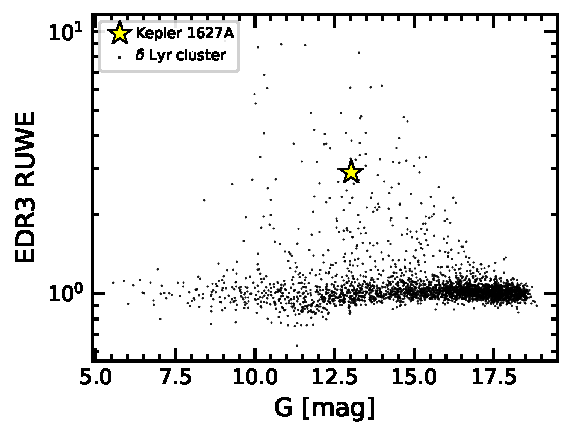
\includegraphics[width=1\textwidth]{f6.pdf}
% 	\end{center}
% 	\vspace{-0.7cm}
% 	\caption{
%     {\bf Galactic position and tangential velocities of the
%     $\delta$\,Lyr cluster.}
%     Points are candidate cluster members with $\varpi/\sigma_\varpi >
%     20$, reported to be in the group by
%     \citet{kounkel_untangling_2019}.  We focus on stars (black points)
%     in the spatial and kinematic vicinity of Kepler\,1627 (yellow
%     star).  The other candidate cluster members (gray points) may or
%     may not share the ages of the selected kinematic group.  The
%     location of the Sun is ($\odot$) is shown.
% 		\label{fig:XYZvtang}
% 	}
% \end{figure*}
% 
% Figure~\ref{fig:XYZvtang} shows stars reported by
% \citet{kounkel_untangling_2019} to be in the group ``Theia 73'', which
% was cross-matched by Kounkel \& Covey as being ``Stephenson 1''.
% \citet{kounkel_untangling_2019} reported \noriginal\ stars to be
% present in this cluster.  For our Figure, galactic positions were
% calculated and plotted only for stars with parallax signal-to-noise
% exceeding 20.  The location of the Sun is shown on the plots.  The
% smattering of reported cluster members (gray and black points) has a
% significantly different structure than the cluster initially
% identified by \citet{stephenson_possible_1959} and corroborated by
% \citet{eggen_photometric_1968}.  While the non-uniform ``clumps''
% might be part of a real structure, they could also be an artifact of
% the data processing steps performed by
% \citet{kounkel_untangling_2019}.  We therefore opted to only consider
% stars in the immediate kinematic and spatial vicinity of \sn.  The
% tangential velocities relative to \sn\ are shown in the bottom right
% panel.  These are computed by assuming that every star has the same
% three-dimensional spatial velocity as \sn, where we assume a systemic
% radial velocity of $-16.7 \pm 0.2$\,\kms\ based on the HIRES
% spectra.  The
% relevant projection effects are then taken into account, as discussed
% by {\it e.g.}, \citet{Meingast2021} and \citet{bouma_2021_ngc2516}.
% We performed the actual selection by then manually drawing lassos with
% the interactive \texttt{glue} visualization tool
% \citep{beaumont_2014_13866} in the four projections shown in
% Figure~\ref{fig:XYZvtang}.  While other cluster members likely exist
% outside of our selection region (and our selection also includes some
% field star interlopers), our aim is to verify the existence of the
% cluster in the vicinity of Kepler\,1627, and to measure its age.  The
% procedure we have adopted enables both tasks.


% \section{Binarity and Stellar Rotation for $\delta$\,Lyr Cluster Members}
% \label{app:rotationbinarity}
% 
% \begin{figure}[t]
% 	\begin{center}
% 		\leavevmode
% 		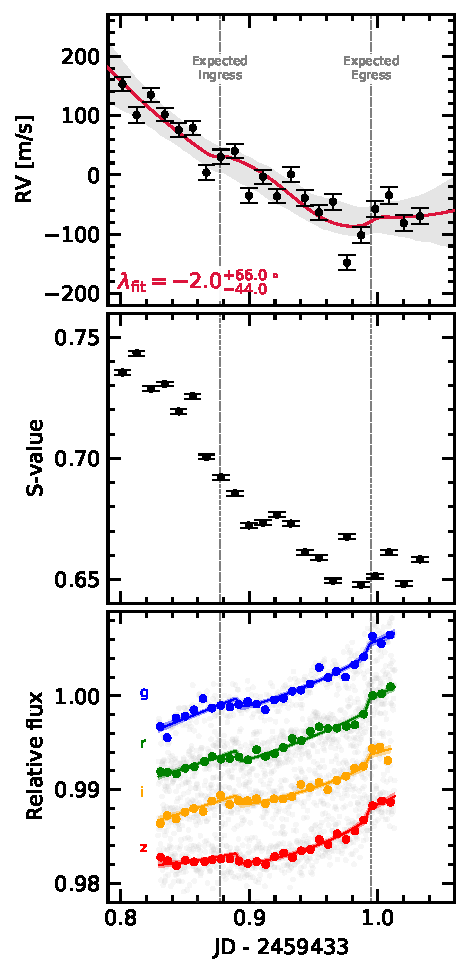
\includegraphics[width=0.7\textwidth]{f7.pdf}
% 	\end{center}
% 	\vspace{-0.7cm}
%   \caption{ {\bf Binarity indicators for rotators in \cn.} 
%     Data are as in the lower panel of Figure~\ref{fig:age}.  Sources
%     with $\mathrm{RUWE}>1.2$ appear in red; these include astrometric binaries as well
%     as sources poorly fit by a single-star PSF.  Photometric binaries
%     ($>$0.3\,mag above an empirical isochrone; 20\% of stars) are
%     orange.  Over $0.6<\bpmrpo<1.5$, the detected rotation periods in
%     binaries tend to fall below the slow sequence.
% 		\label{fig:binarity}
% 	}
% \end{figure}
% 
% Figure~\ref{fig:binarity} shows the rotation-color diagram for \cn\
% members, with the points colored according to indicators of binarity.
% The binaries tend to be redder and have shorter rotation periods.  We
% know of two possible explanations based on selection effects, and two
% based on physics.
% 
% Possible selection effects include {\it i)} binaries have a component
% that contributes additional red light to the system, which could skew
% the color measurement of the primary; and {\it ii)} the unresolved
% binary companions could contaminate the rotation period measurement
% \citep[{\it e.g.},][Section~5.1]{stauffer_rotation_2016}.
% 
% The two possible physical effects that could be relevant are tidal
% locking and pre-main-sequence disk locking.  Tidal locking has been
% argued to be an unlikely explanation for the frequency of rapid
% rotators due to the population statistics; a more likely scenario
% would be that the presence of the binary leads to faster disk
% dispersal, enabling the primary to contract to more rapid rotation
% periods than possible for single stars
% \citep{meibom_effect_2007,bouma_cluster_2020}.



\section{The Transit Asymmetry}
\label{app:asymmetry}

\begin{figure}[t]
	\begin{center}
		\leavevmode
		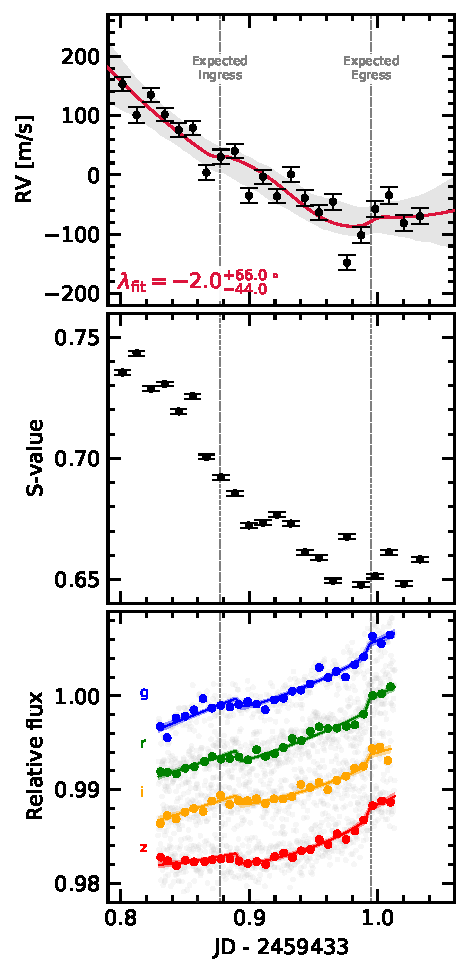
\includegraphics[width=0.64\textwidth]{f7.pdf}
	\end{center}
	\vspace{-0.7cm}
	\caption{
		{\bf Transit model residuals through time (binned by Kepler quarter)}.  
    {\it Left:}
    Phase-folded transit of Kepler 1627b, with stellar variability
    removed.  Black points are binned to 20
    minute intervals.  The 2-$\sigma$ model uncertainties and the
    maximum {\it a posteriori} model are shown as the faint purple
    band, and the dark purple line.
    {\it Right:}
    As on the left, with the transit removed.  Quarters 6 and 7 show a
    consistent deviation in the second half of the transit.
		\label{fig:phasequarter}
	}
\end{figure}

\begin{figure}[t]
	\begin{center}
		\leavevmode
		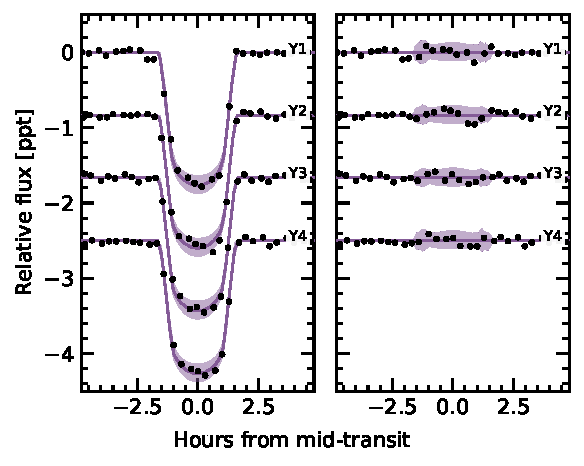
\includegraphics[width=0.64\textwidth]{f8.pdf}
	\end{center}
	\vspace{-0.7cm}
	\caption{
    {\bf Transit model residuals through time (binned by year of observation)}.  
    {\it Left:}
    Phase-folded transit of Kepler 1627b, with stellar variability
    removed.  Points and models are as
    in Figure~\ref{fig:phasequarter}.
    {\it Right:}
    As on the left, with the transit removed.
		\label{fig:phaseyear}
	}
\end{figure}

\begin{figure}[t]
	\begin{center}
		\leavevmode
		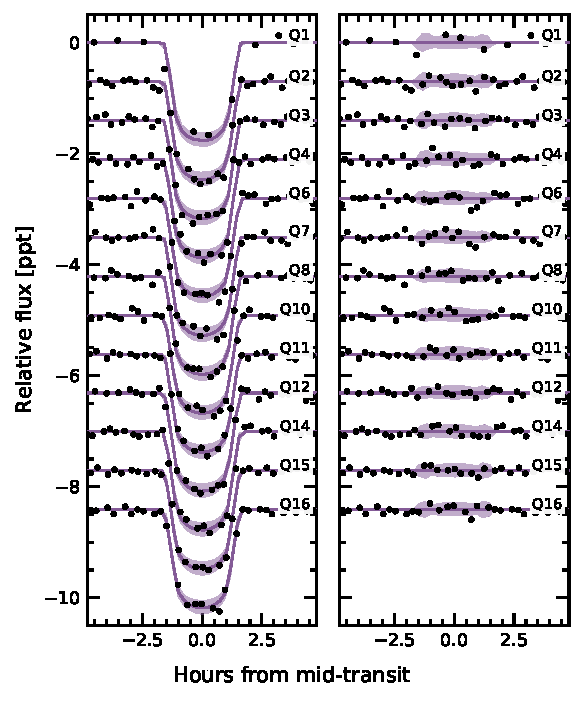
\includegraphics[width=\textwidth]{f9.pdf}
	\end{center}
	\vspace{-0.7cm}
	\caption{
    {\bf Transit models and residuals, binned by local slope of the
    raw light curve}.  Local linear slopes are measured over each
    transit window (144 transits total).  Four outlier transits were
    removed, leaving 140 transits.  These were then divided into
    quartiles, so that each panel shows 35 transits binned together.
    The exact light curve slopes are listed in the lower left panels.
    Representative uncertainties for the black points (binned at 20
    minute intervals) are shown in the lower right of each panel.  A
    similar transit asymmetry to that shown in Figure~\ref{fig:lc}
    seems to be present in three of the four bins.
		\label{fig:phaseslope}
	}
\end{figure}


As a means of exploring the robustness of the transit asymmetry,
Figures~\ref{fig:phasequarter},~\ref{fig:phaseyear},
and~\ref{fig:phaseslope} show the Kepler data binned in three ways:
over quarters, years, and local slope quartiles.  Over quarters
(Figure~\ref{fig:phasequarter}), Quarter 6 shows the strongest asymmetry
out of any quarter: a deviation of about 3\,ppt from expectation.
Quarter 7 shows an anomaly at roughly the same transit phase.  Year 2
correspondingly shows the strongest anomaly out of any year in
Figure~\ref{fig:phaseyear}; the asymmetry is visually apparent however
in each of Years 2, 3, and 4.
Binned by local slope quartiles (Figure~\ref{fig:phaseslope}), the
asymmetry is visually present in three of the four quartiles: the only
bin for which it appears to not be present is ${\rm d}f/{\rm
d}t\in[0.001,0.033]\,{\rm ppt\,day}^{-1}$.

We considered four possible interpretations of the transit asymmetry:
gravity darkening, transit timing variations, spot-crossing events,
and a persistent asymmetric dusty outflow.  

Gravity darkening is based on the premise that the rapidly rotating
star is oblate, and brighter near the poles than the equator
\citep[{\it e.g.},][]{masuda_spin-orbit_2015}.  The fractional transit
shape change due to gravity darkening is on the order of $(P_{\rm
break}/P_{\rm rot})^2$, for $P_{\rm break}$ the break-up rotation
period, and $P_{\rm rot}$ the rotation period.  Using the parameters
from Table~\ref{tab:posterior}, this yields an expected 0.14\%
distortion of the $\approx$1.8\,ppt transit depth: {\it i.e.}, an
absolute deviation of $\approx$2.5\,ppm.  The observed residual has a
semi-amplitude of $\approx 50\,{\rm ppm}$.  Since the expected signal
is smaller than the observed anomaly by over an order of magnitude,
gravity darkening seems to be an unlikely explanation.

The scenario of transit timing variations (TTVs) producing the
asymmetry seems unlikely because our analysis showed that transit
timing variations in \sn\ have amplitudes smaller than $\approx$10
minutes (see Figure~\ref{fig:corr}).  This is consistent with
previous results from \citet{holczer_transit_2016}.  Moreover, the
transit timing variations we do observe are correlated with the local
light curve slope, which on average increases as much as it decreases.
From our analysis, the mean TTV and its standard deviation are
$0.00\pm12.05$ minutes; similarly the mean local slope and its
standard deviation are $0.49\pm44.49$\,ppt\,day$^{-1}$.  There is
therefore no expectation for TTVs to produce the asymmetry.  A
separate line of argument comes from Figure~\ref{fig:phaseslope}.  If
the local slope were essential to producing the transit asymmetry, we
would expect that in the largest ${\rm d}f/{\rm d}t$ bin, ${\rm
d}f/{\rm d}t\in[0.033,0.092]\,{\rm ppt\,day}^{-1}$, the sign of the
asymmetry would reverse.  We do not see evidence for this being the
case.

The third and related possibility is that of starspot crossings.
Young stars have higher spot-covering fractions than old stars ({\it
e.g.}, \citealt{morris_relationship_2020}).  Young solar-type stars
may also host dark starspots at high stellar latitudes \citep[{\it
e.g.}, EK~Dra;][]{strassmeier_starspots_2009}, though interferometric
imaging of spotted giant stars has shown different starspot latitude
distributions than those inferred from Doppler imaging
\citep{roettenbacher_contemporaneous_2017}.  Regardless, for any
spot-crossing anomalies to add coherently over the 144 Kepler
transits, it seems likely that we would need either for spots to be
persistent at a particular latitude (and for the planetary orbit to be
somewhat misaligned), or for a ``stroboscopic'' longitudinal phasing
\citep[{\it e.g.},][]{dai_stellar_2018}.  For our system, $P_{\rm
orb}/P_{\rm rot} \approx 2.76$, which means that every 4 transits and
11 stellar rotations, the planet crosses over roughly the same stellar
longitude, which might enable the necessary phasing if the spot-groups
are large and long-lived.  Unfortunately, the  S/N per Kepler transit
is $\approx8$, which renders individual spot-crossing events
unresolved.  This explanation seems marginally plausible, mainly because the
expected spot-crossing anomaly amplitudes ($\approx 100\,{\rm ppm}$)
resemble the observed amplitude of the asymmetry ($\approx 50\,{\rm
ppm}$).
One issue with this explanation however is that
there is no reason to expect starspot crossing events to last
exactly half the transit duration.

A persistent feature of the planet itself might therefore be needed to
explain the transit asymmetry.  An asymmetric outflow from the
planet's atmosphere could at least geometrically meet the requirements
\citep[{\it e.g.},][]{mccann_2019}.  To explain the asymmetric
transit, a small, dense component would lead the planet, and a long,
more rarefied (and variable) component would trail it.  This might
also explain the slight flux decrement visible for $\sim$1 hour
pre-ingress (Figure~\ref{fig:lc}).  The amplitude of the asymmetry is
roughly in line with theoretical expectations for dusty outflows
\citep{wang_dai_2019}, and based on the planet's size, its mass is
likely in a regime where such outflows are possible.  Out of the four
explanations discussed, this one at least theoretically seems the most plausible.
By composition, the expectation would be that the envelope is mostly
hydrogen and helium gas, with a dust or haze component providing the
broadband opacity in the Kepler bandpass.  A natural path
toward confirming or refuting this idea would be to observe additional
transits of the planet in hydrogen absorption, 
metastable helium absorption, or across a broad wavelength range in
the near-infrared.


%  \subsection{Short Cadence Data}
%  
%  \begin{figure*}[t]
%  	\begin{center}
%  		\leavevmode
%  		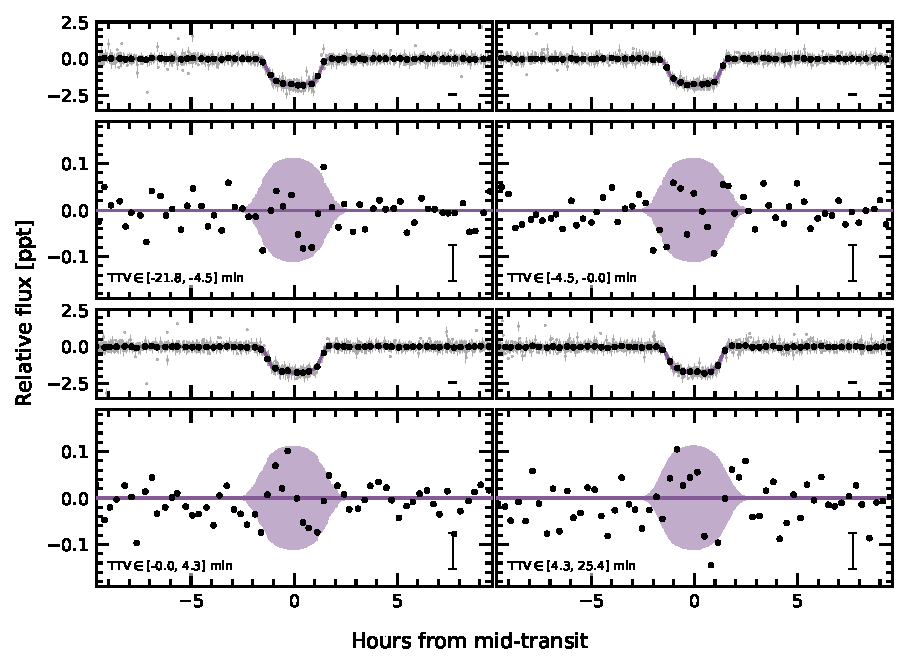
\includegraphics[width=1\textwidth]{f12.pdf}
%  	\end{center}
%  	\vspace{-0.7cm}
%  	\caption{
%  		{\bf Phase-folded short cadence transit of Kepler\,1627 Ab}.  
%      The precision with which the impact parameter can be measured is
%      higher than from the long cadence data.
%  		\label{fig:phase_slc}
%  	}
%  \end{figure*}
%  
%  Figure~\ref{fig:phase_slc} shows the result from analyzing 100 days of
%  short cadence (1-minute) data acquired during Quarter 15.
%  %TODO: get quantitative on better impact parameter...






\section{Spectroscopic Transit Analysis}
\label{app:rm}

\begin{figure*}[tp]
	\begin{center}
		\leavevmode
		\subfloat{
			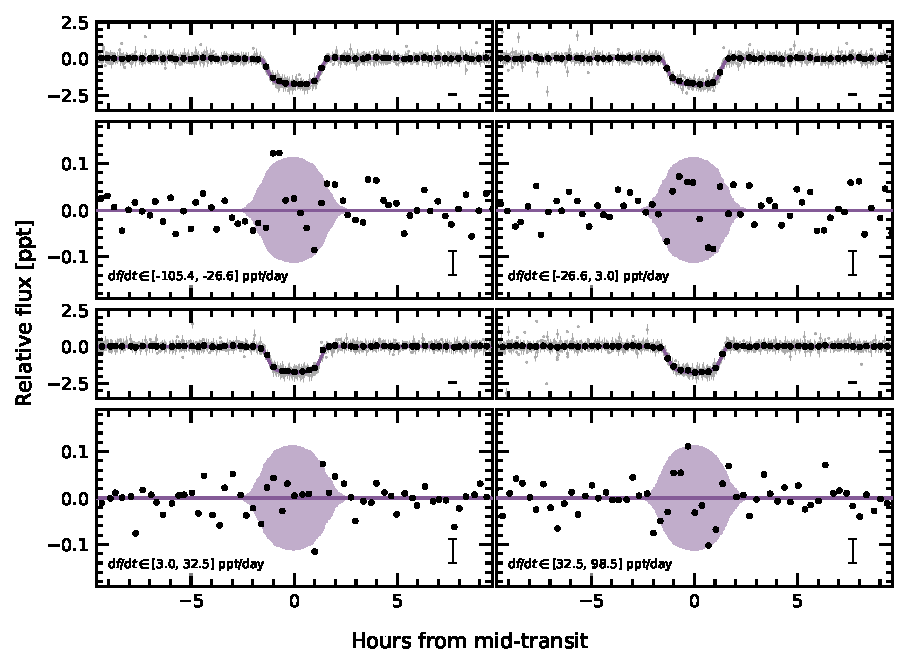
\includegraphics[width=\textwidth]{f11.pdf}
		}
	\end{center}
	\vspace{-0.5cm}
	\caption{
    {\bf Spectroscopic activity indicators during the transit of 2021
    Aug 7.} The {\it top panels} show the median line profiles Ca K,
    Ca H, and H$\alpha$ line profiles from the HIRES spectra.  The
    {\it lower panels} show the differences of each individual
    spectrum relative to the median spectrum.  The bump in the red
    wing of Ca H is H$\epsilon$.
    The spectra in the lower panels are smoothed for visualization
    purposes.
    \label{fig:rvactivity}
	}
\end{figure*}

We monitored \sn\ with Keck/HIRES before, during, and after transit on
the night of 2021 Aug 7.  We used the iodine cell for wavelength
calibration\footnote{We considered a line-profile based analysis in
the regions without iodine, but the line profile stability of HIRES
precludes such an approach.}, extracted the 1-D spectra using the
standard California Planet Survey pipeline \citep{howard_cps_2010},
and measured the velocities by cross-correlating against a template
found via spectral classification with \texttt{SpecMatch-Emp}
\citep{yee_SM_2017}.  The airmass ranged between 1.1 and 2.2 from the
start through the end of observations; the seeing ranged from
$1\farcs1$ at the beginning to $1\farcs5$ at the end.  We also
simultaneously observed across {\it griz} bands using MuSCAT3 at
Faulkes Telescope North on Maui, HI.

Figure~\ref{fig:ground} shows the results.  The
MuSCAT3 photometry shows the expected starspot trend, along with the
transit and what is likely a chromatic starspot crossing event at
${\rm JD} - 2459433 = 0.955$.  The radial velocities decrease by
800\ms\ over the six hour window.  A $\approx50$\ms\  increase in RV
is seen shortly after the expected ingress time. 

Overall, we expect the dominant trends in both the photometry and
radial velocities to be caused by starspots on the stellar photosphere
rotating into and out of view.  The plasma in the leading and receding
limbs of the stellar disk has an apparent line-of-sight velocity of
$\pm 20$\kms.  Over 10\% of a rotation cycle ($P_{\rm
rot}=2.6\,{\rm days}$), spots near these limbs come into and out of
view, modulate the stellar velocity profile, and can thereby produce
the overall 800\ms\ trend.  The Ca HK and H$\alpha$ emission
profiles support this interpretation;
Figure~\ref{fig:rvactivity} shows that each line gradually decreases in
intensity over the course of the six hour sequence.
The overall RVs are also heavily correlated against the S-indices
derived from the Ca HK lines.

The expectation however is for the starspot-induced signals to be smooth,
at worst with contributions at $0.5\,P_{\rm rot}$ or $0.25\,P_{\rm
rot}$ \citep{klein_simulated_2020}.  We therefore fitted the RVs using
the \citet{hirano_analytic_2010,hirano_2011} models for the
Rossiter-McLaughlin (RM) effect, and allowed for an optional linear
and quadratic trend in time to fit the 800\ms\ spot-induced trend.  We
followed the methodology developed by \citet{stefansson_2020}.  We
allowed the sky-projected obliquity, the projected stellar equatorial
velocity, and the Gaussian dispersion of the spectral lines to vary,
and fixed the limb-darkening using the $V$-band tabulation from
\citet{claret_gravity_2011}.  We assumed a prior on $v\sin i$ and
$a/R_\star$ from Table~\ref{tab:starparams}, and also allowed for a
white-noise jitter term to be added in quadrature to the measurement
uncertainties.

The quadratic model with the RM effect is shown in
Figure~\ref{fig:ground}; the jitter term is incorporated in the
model uncertainties, but not the plotted measurement uncertainties.
The plotted measurement uncertainties are the internal uncertainties
on the RVs ($\approx 15\,{\rm m\,s}^{-1}$), and are dominated by the
$v\sin i$ broadening.  However, between exposures, the RVs show
significant additional scatter that is not captured by the slow quadratic
trend.  The white-noise jitter for this
particular model is $\sigma_{\rm RV} = 50^{+11}_{-8}$\ms, which is
larger than the expected RM anomaly of $\Delta v_{\rm RM}
\approx f_{\rm LD} \cdot \delta \cdot v\sin i \cdot \sqrt{1-b^2}
\approx 20\,{\rm m\,s}^{-1}$.

The presence of this additional scatter prevents a convincing detection of
the RM effect.  The reason can be understood via
model comparison.  If we compare the model with a quadratic trend and
the RM effect against a model with a
linear trend and the RM effect, or even a model with no RM effect at
all, then the respective Bayesian Information Criterion (BIC) values
are as follows.
% from logs/rm_freejitter_FINAL.log
\begin{align}
  {\rm BIC} &= 251.7  \quad ({\rm Quadratic+RM}) \nonumber \\
  {\rm BIC} &= 257.7  \quad ({\rm Linear+RM}) \nonumber \\
  {\rm BIC} &= 247.1  \quad ({\rm Only\ Quadratic}).
\end{align}
There is therefore no evidence to prefer the model with the RM effect
against a model that only accounts for the stellar variability.
The ``only quadratic'' model does particularly well because it can
inflate the jitter term to account for scatter during
the transit (even if the scatter contains astrophysics!), and it has fewer free parameters.  However, we cannot
justify a physical prior on the jitter term, because we do not
understand the origin of the exposure-to-exposure scatter.  As noted
above, the velocity deviations from starspots are expected to have
contributions at the stellar rotation frequency, or harmonics thereof.
This jitter is present on the exposure timescale (15 minutes), which
is only 0.4\% of the stellar rotation period; it is not obvious that
starspots would be the culprit.

The amplitude of both the spot-induced trend and the jitter are larger
than recent comparable measurements in systems such as AU~Mic
\citep{palle_transmission_2020}, DS~Tuc
\citep{montet_young_2020,zhou_well_2020} and TOI~942
\citep{wirth_2021_toi942}.  One possible explanation for the jitter is
that it is astrophysical in origin, and that it is caused by some
novel process operating on the surface of Kepler 1627A.  Another
possibility is that our RV analysis underestimates the measurement
uncertainties; the S/N per resolution element for each of our spectra
was moderated by the observing requirements to 70 to 80, and the rapid
rotation of the star could affect accuracy of the uncertainties from
the velocity extraction.  Observations at higher precision are
necessary to distinguish these two possibilities, and remain
worthwhile as a means toward clarifying the orbital geometry of \pn.




\section{Flare Analysis}
\label{app:flare}

In addition to the 3.9 years of long cadence data, short cadence
(1-minute) Kepler observations were acquired over 97.7 days during
Quarter 15.  The short cadence light curve shows a higher rate of
flaring than visible in the long cadence data
(Figure~\ref{fig:flarezoom}).  We analyzed the short cadence light
curve and its flares according to the following procedure.
\begin{enumerate}
  \item Fit the starspot-induced variability using a
    Gaussian Process with a \texttt{SHOTerm} kernel, a white-noise jitter term, and the
    mean flux.
  \item Select points more than twice the median absolute
    deviation from the residual, and exclude them from the light
    curve (these points include the flares).  Repeat Step~1.
  \item Using the residual from Step 2, identify all flares,
    requiring them to be at least 20 cadences apart, at least 7 median
    absolute deviations above the median baseline, and lasting at
    least 2 cadences in duration.  Build the mask spanning these
    times, from 5 minutes before each flare begins to 2.5 minutes
    after the final flare cadence.  Repeat Step 1 a final time.
\end{enumerate}
The final step of flare identification and fitting was performed using \texttt{altaipony}
\citep{davenport_2016,ilin_flares_2021}.  The analytic flare model is
from \citet{davenport_2014} and it parametrizes the flare with a start
time, an exponential lag time, and an amplitude.
%Figure~\ref{fig:flarephase} shows the resulting flares, amplitudes,
%and phases.

\begin{figure*}[tp]
	\begin{center}
		\leavevmode
		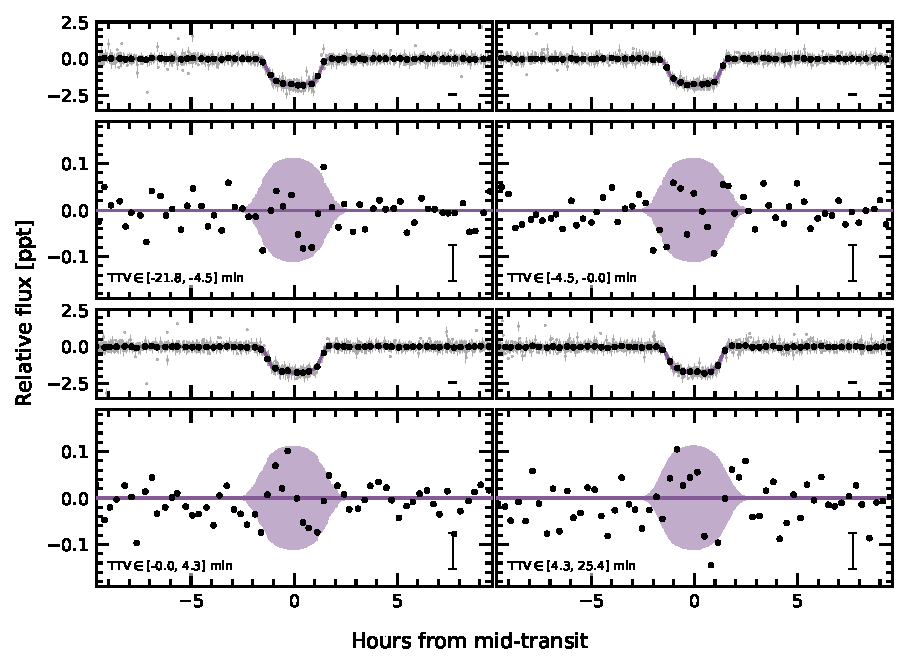
\includegraphics[width=0.9\textwidth]{f12.pdf}
	\end{center}
	\vspace{-0.7cm}
	\caption{
		{\bf Flares in Kepler\,1627}.  
		{\it Top:}
		The full short cadence Kepler dataset, acquired at 1-minute
		sampling (black points) is shown with a stellar variability model
		(blue line).
		{\it Middle:}
		Residual after subtracting the stellar variability model.  Flares
		appear as spikes.
		{\it Bottom:}
		Zooms of the brightest, and third-brightest flares.  A timing
		coincidence -- that both flares have ``successors'' approximately
		one orbital period after the initial event -- is emphasized.
		\label{fig:flarezoom}
	}
\end{figure*}

%\begin{figure*}[t]
%	\begin{center}
%		\leavevmode
%		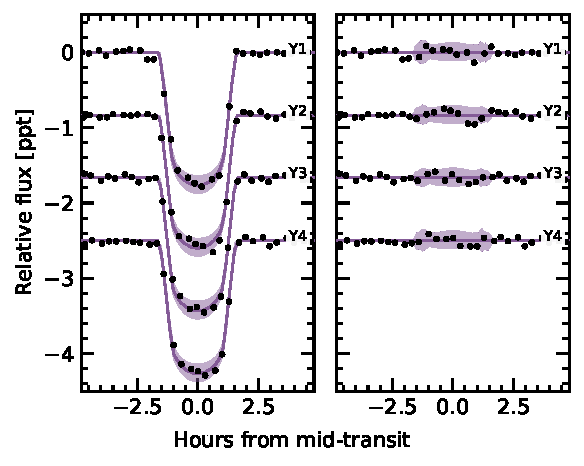
\includegraphics[width=0.9\textwidth]{f8.pdf}
%	\end{center}
%	\vspace{-0.7cm}
%	\caption{
%		{\bf Phase-folded flares in Kepler\,1627}.  
%    {\it Top:}
%    As in the middle of Figure~\ref{fig:flarezoom}, phase-folded at
%    the planet's ephemeris.
%    {\it Bottom:}
%    Fitted flare amplitudes and orbital phases -- each point
%    represents one flare.
%    Colors indicate relative time, from the beginning of the
%    98-day short cadence Quarter 15 dataset (dark blue) to the end (light
%    yellow).
%    Lower amplitude flares likely exist in the data, and were not
%    examined.
%		\label{fig:flarephase}
%	}
%\end{figure*}

\begin{figure*}[tp]
	\begin{center}
		\leavevmode
		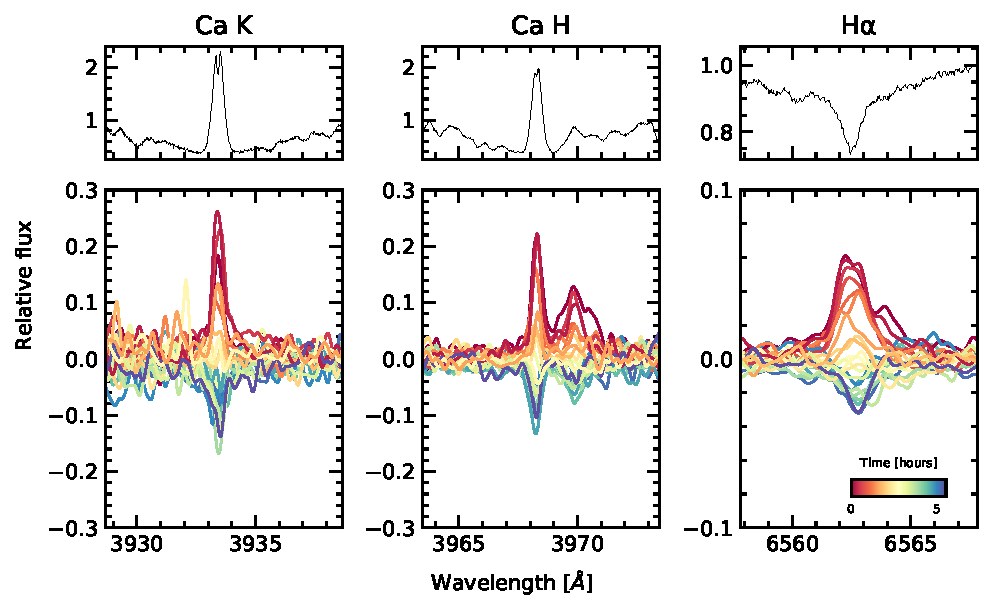
\includegraphics[width=0.8\textwidth]{f13.pdf}
	\end{center}
	\vspace{-0.7cm}
	\caption{
		{\bf Statistics of inter-flare arrival times}.  
    24 flares were recorded with amplitudes exceeding 0.5\% over the
    97.7 days of short cadence observations.  The histogram of the
    time intervals between every possible pair of flares is shown in
    black.  Some plausibly important timescales for star-planet
    interactions, namely the planetary orbital period and synodic
    period (the orbital period as seen from the rotating stellar
    frame) are shown along with their linear combinations.  Monte
    Carlo draws from a Poisson distribution are shown with the gray
    bands.  While peaks in the observed distribution do coincide with
    some of the ``special periods'', the statistical evidence for a
    non-Poissonian process driving the flares does not reach the
    $5$-$\sigma$ threshold.
		\label{fig:flarestats}
	}
\end{figure*}


There were $N_{\rm f}=24$ flares that exceeded $0.5\%$ in relative
flux during the short cadence observations.  These 24 flares spanned a
total of 6.5 hours ($\sim$15 minutes per flare).  Inspecting the data,
we noticed a coincidence in the flare arrival times.  The coincidence
is that despite the low flare duty cycle, one orbital period after the
brightest flare, a second flare followed.  This and a similar event
are shown in Figure~\ref{fig:flarezoom}.  The timing error is good to
a $\approx0.2\%$ difference from the orbital period, which given the
duty cycle seems {\it a priori} unlikely.  If we consider flares
falling within 2\% of the planet's orbital period after a previous
flare, then 4 of the 24 flare events have candidate ``successors''.

As with any coincidence, if one does not have a firm prediction, it is
difficult to assess whether a surprise is statistically significant.
Since our surprise was specifically at the inter-arrival time of
certain flares coinciding with special time intervals, we performed
the following analysis.  First, we considered all unordered pairs of
flares.  For $N$ flares there are ${n \choose 2}$ such pairs (for our
case, 276 pairs).  We then compared the distribution of the pair
separations against that of a Poisson distribution.  Specifically, we
drew $N_{\rm f}=24$ samples from a Poisson distribution with $\lambda
= \Delta t / N_{\rm f}$, for $\Delta t=97.7\,{\rm days}$ the total
duration of the observations, and repeated the draw $10^3$ times with
unique random seeds.

Figure~\ref{fig:flarestats} shows the results.  The vertical lines in
the figure show the planetary orbital period, the synodic period
$P_{\rm syn} = (P_{\rm rot}^{-1} - P_{\rm orb}^{-1})^{-1}$, and linear
combinations thereof.  The tidal period (half the synodic period) is
not shown.  The bins are logarithmically spaced to give 100 bins
between the minimum and maximum ordinate values.  The gray bands
express the range of values observed from the Poissonian draws.  While
it does seem like an odd coincidence for peaks in the observed flare
arrival time distribution to coincide with the locations of these
``special intervals'', the statistical evidence for a non-Poissonian
process driving the flares does not seem especially overwhelming.
More quantitatively, the peaks observed at the orbital and synodic
periods are within the $\pm 2$-$\sigma$ range of a Poissonian process,
and those at $P_{\rm orb}+P_{\rm syn}$ and $P_{\rm orb}+2P_{\rm syn}$
are only slightly above this range.  With that said, future analyses
of these data by investigators with more knowledge of this topic could
very well yield more quantitative insights.  Such analyses should keep
in mind an important caveat: the amplitude distribution of M-dwarf
flares extends up to many times the quiescent flux \citep[see Figure~7
of][]{gunther_2020}.  A flare on Kepler\,1627B producing double its
quiescent white-light flux would yield a $\approx$1\% apparent
amplitude.  Such flares could represent a significant fraction of
those in the Kepler observations.





\listofchanges

%\allauthors
\end{document}
